\documentclass[12pt,a4paper,twoside,openany]{report}

\usepackage{graphicx}
\usepackage{amsmath}
\usepackage{amsthm}
\usepackage{amssymb}
\usepackage{listings}
\usepackage{xcolor}
\usepackage{textcomp}
\usepackage{setspace}
\usepackage[final]{pdfpages}
\usepackage{lscape}
\usepackage{cite}
\usepackage[toc,page]{appendix}
\usepackage{epstopdf}
\usepackage{multicol}
\usepackage[includeheadfoot, margin=3cm]{geometry}
\usepackage{fancyhdr}
\usepackage{url}
\usepackage{lscape}
\usepackage{rotating}
\usepackage{booktabs}
\usepackage{float}
\usepackage{cancel}
\usepackage[framed,numbered,autolinebreaks,useliterate]{mcode}
\usepackage[colorlinks=false,pdfborder={0 0 0}]{hyperref}
\usepackage{placeins}
\usepackage[utf8]{inputenc}
\usepackage[T1]{fontenc}
\usepackage{lmodern}
\usepackage{breqn}
\usepackage{titlesec}
\usepackage{pdfpages}

\usepackage{draftwatermark}
\SetWatermarkLightness{0.95}

\bibliographystyle{plain}
% Figures within a column...
\makeatletter
\newenvironment{tablehere}
{\def\@captype{table}}
{}
\newenvironment{figurehere}
{\def\@captype{figure}}
{}
\makeatother
  
%commands
\providecommand{\e}[1]{\ensuremath{\times 10^{#1}}}

% Document properties
\hypersetup{pdfauthor={Stephen Wardrop},pdftitle={Honours Thesis}}

% Set figure numbering
\renewcommand{\thefigure}{\arabic{chapter}.\arabic{figure}}
\renewcommand{\theequation}{\arabic{chapter}.\arabic{equation}}
\renewcommand{\thetable}{\arabic{chapter}.\arabic{table}}

\renewcommand{\chaptermark}[1]{\markleft{}}
\renewcommand{\sectionmark}[1]{\markright{}}

\begin{document}
% Title page
\thispagestyle{empty}
\begin{titlepage}
\setcounter{page}{1}
\begin{center}

\begin{figure}[H]
\centering

\includegraphics[width = 0.8\textwidth]{Images/usyd.jpg}
\end{figure}

\doublespacing
\textsc{ \LARGE Algorithm Design for Real-Time Path Planning of Underactuated Dynamic Walking Using Virtual Constraints}

\vspace{2cm}

\singlespacing
A thesis submitted in partial fulfilment of the requirements for the degree of \\ Bachelor of Engineering (Honours) and Bachelor of Science

\vspace{2cm}

\large
Stephen Wardrop

\vfill

October, 2014

\end{center}
\end{titlepage}
\pagebreak

\begin{abstract}
\thispagestyle{plain}
\pagenumbering{roman}
\setcounter{page}{2}
There is significant interest, both technical and aesthetic, in developing bipedal robots which locomote stably, efficiently and reliably over uneven terrain. This continues to present a significant challenge due to computational intractability, highly complex nonlinear dynamics and intrinsic static and dynamic instability. Successful methods which achieve walking gaits restrict the problem to particular domains or motions to overcome the intractability of the general problem. One such method is to prepare a library of motion primitives and thus to limit the on-line computation to the choice of a particular constraint within the library. \\

Previous work has demonstrated the in-principle effectiveness of the motion primitives approach for real-time path planning of dynamic walking over uneven terrain. The contribution of this thesis work is to present a general method for the production of a library of motion primitives which achieves sufficient coverage of the feasible motions of the robot along with a method for intelligently choosing between them.
\end{abstract}

\pagebreak

\renewcommand{\abstractname}{Statement of student contribution}
\begin{abstract}
\thispagestyle{plain}
\pagenumbering{roman}
\setcounter{page}{3}
\begin{itemize}
	\item I completed the literature review largely independently, with some papers being recommended to me by my supervisor
	\item I designed and implemented the simulator for the compass-gait robot and 5-link walker, with the code for generating the dynamics of the 5-link walker being sourced from Westervelt et al \cite{westervelt2007feedback}.
	\item I designed the graphical interfaces for the investigation of virtual constraints
	\item I designed the method by which the motion primitives could be automatically generated {\color{red}(yet to complete...)}
	\item I extended the algorithm designed by my supervisor and others to include a more intelligent heuristic for selection of motion primitives in real time. {\color{red}(yet to complete...)}
\end{itemize}
~\\~\\

The above represents an accurate summary of the student's contribution.  \\~\\~\\

Signed \\~\\~\\

_______________ (student) \hspace{5mm} _______________ (supervisor)
\end{abstract}

\pagebreak

\renewcommand{\abstractname}{Acknowledgements}
\begin{abstract}
\thispagestyle{plain}
\pagenumbering{roman}
\setcounter{page}{4}
I would like to thank my supervisor, Dr Ian Manchester, for his time and forbearance in helping me grasp the matter of this field. Along with him, I thank Jack Umemberger for his helpful comments and insights to get me up to speed with his previous work in this matter. \\

I thank <anybody who did this> for proofreading and advice given. \\

I also thank my wife for enduring the countless nights and weekends spent with a preoccupied or absent husband even while taking care of our young daughter. Your encouragement and patience have been vital.
\end{abstract}


\pagenumbering{roman}
\setcounter{page}{5}
\tableofcontents
\listoffigures
\listoftables
\clearpage

\fancyhf{}
\pagestyle{fancy}
\fancyhead[LE]{\textit{\leftmark}}
\fancyhead[RO]{\textit{\rightmark}}
\fancyhead[RE,LO]{Stephen Wardrop}
\fancyfoot[CE,CO]{\thepage}
\pagenumbering{arabic}
\setcounter{page}{1}
\onehalfspacing

\begingroup
\titleformat{\chapter}[display]
	{\bfseries\Large}
	{}
	{1ex}
	{\titlerule\vspace{1ex}
	\ifnum\value{chapter}>0 \MakeUppercase{\chaptertitlename}~\Huge\thechapter \fi
		~ \Large\filright}
	[\vspace{1ex}\titlerule]

\chapter{Introduction}
\setcounter{figure}{0}\setcounter{equation}{0}\setcounter{table}{0}
Motivated by the dexterity, terrain scalability and reach availed to humans through the use of legs, and for social and aesthetic reasons, robotics researchers have sought to create humanoid robots. While there are notable examples of significant success in this endeavour, the motion characteristics of these robotic walkers are noticeably different from our own. This is largely due to the restricting of the robotic systems to full actuation, which permits convenient simplifications and robustness. This restriction imposes more than simply visual differences; the conservative motion restricts the speed at which these robots can move and, importantly, their efficiency. Consequently, there exists interest in developing underactuated robotic walkers which utilise the dynamics of the system to generate much of the motion, imposing actuation only where required to enforce a trajectory or respond to disturbance.

However, permitting underactuation causes the path planning and control problems to become significantly more complex. This is mainly due to two contributing factors. Firstly, the dynamics of walking robots are highly nonlinear, particularly about the foot impacts, and so the system model must be very complex or else be a poor approximation. Secondly, the search space to find feasible paths is vast, since in general robotic walkers have many independent degrees of freedom, making traditional methods of planning and control computationally intractable. In addition, control problems of underactuated and fully actuated control are sufficiently different that much of the intuition and methods from the quite well studied field of fully actuated control are not easily applicable to underactuated cases.

Manchester et al \cite{manchester13planning} have proposed a method for path planning for underactuated dynamic walkers using a receding-horizon algorithm which draws from a library of motion primitives defined as virtual holonomic constraints to address the above mentioned challenges. The use of a library of motion primitives drastically reduces the search space and notionally limits the trajectories to feasible motion. The complications regarding the nonlinear impact dynamics are isolated by defining of motion primitives by the duration of one continuous phase – that is, the movement of the robotic walker between one foot impact and the next. Also, the use of virtual holonomic constraints allows for a partial closed-form solution of the dynamical equations to be computed off-line, thereby significantly reducing the required on-line computation in determining dynamic feasibility. This method has been proven to be capable of planning several footsteps ahead of the current position of the robot in a fraction of a second, thus being feasible for real-time control, on a compass-gait walker and more complex 5-link walker.

Power and energy densities pose strict limits on the dimensions and weight of walking robots with present technology. Additionally, ethical considerations in sustainable design guide us to minimise wasteful energy consumption. There are two applicable means by which the energy consumption of an underactuated walking robot may be reduced in the context of motion planning: Minimising the actuator energy output and reducing the computational requirements of the planning algorithm. The virtual constraints approach provides a convincing means of achieving the latter, however the ability of this approach to produce paths close to the true optimal in terms of energy reduction is dependent upon the optimality and coverage of the motion primitives within the library and the manner by which one primitive is preferred over another.

\section{Problem Statement}
In the light of these motivations, the primary aim of this thesis is to produce a method by which optimal primitives may be generated in a procedure which ensures sufficient coverage of the configuration space of the robot. This library is structured to enable rapid traversal in real-time. In addition, an algorithm by which the primitives may be selected rapidly and intelligently is implemented. The combination of these two components enable efficient real-time path planning of underactuated dynamic walkers.

\section{Structure of thesis}
This thesis builds on the work completed by Manchester \& Umenberger \cite{manchester13planning}, which itself arises from a decade of interest in the literature in the method of virtual constraints for control of underactuated walking robots.

\begin{adjustwidth}{1.4cm}{}
\begin{enumerate}[label=\bfseries Chapter \arabic*]
	\setcounter{enumi}{1}
	\item introduces the relevant literature in the planning and control of underactuated robotics, particularly as it applies to walking robots. Particular attention is paid to the method of virtual constraints.
	\item presents the mathematical and technical background required for understanding and applying virtual constraints to underactuated walking robots. In addition, the techniques used for the principled design of virtual constraints as motion primitives are established.
	\item outlines the primary contribution of this thesis work; the method for automatic generation of a library of virtual constraints.
	\item details the planning algorithm, based upon that found in \cite{manchester13planning}, which is used to select a virtual constraint from the library for the purposes of motion planning.
	\item presents the results of testing the validity of the method introduced in Chapter 4, firstly by examining the properties of the virtual constraints themselves and then using a simulator, which is outlined in Appendix \ref{chap:sim}, to assess its efficacy of use in motion planning
	\item discusses the key outcomes raised in Chapter 6 along with the merits of the virtual constraints method
	\item concludes by establishing the contribution of this thesis to the state of the art and outlining the future work required for the application of the methods used in this work in practice to general underactuated walking robots
\end{enumerate}
\end{adjustwidth}
\clearpage

\chapter{Literature Review}
\setcounter{figure}{0}\setcounter{equation}{0}\setcounter{table}{0}
\section{Background}
This work is focused on path planning for underactuated walking robots using virtual holonomic constraints as motion primitives. The objective is to allow for robust real-time approximately-optimal control of underactuated walkers on rough terrain. This is based upon previous work in several fields, including walking robot dynamics, motion planning, the application of virtual constraints in control and path planning and feedback control to enforce the desired trajectories.

Walking robots are a subset of mobile robots. Other common methods of locomotion include wheels, rails and tracks. Walking robots have gathered interest for their ability to traverse terrain which is impassable to these other classes of mobile robot. However, walking robots are typically significantly less efficient and difficult to plan and control in comparison to wheeled robots. In order for legged locomotion to be viable, it must become robust, efficient and rapid. Also, other than for the limited applications in which motion can be pre-planned, it must be computable in real-time.

Feedback control has been a very important field of research in generating robust and useful robots. It has proven exceptionally effective at ensuring robotic motions match planned motions, particularly in systems of sufficiently low dimensionality and complexity. For conventional wheeled and fixed robots, feedback control laws are normally well-understood and behaviour can be prescribed which will be reliably and robustly tracked \cite{rivera1986internal}. However, for legged robots, especially underactuated robots, the required feedback control is not straightforward. There has been a large amount of recent work in analysing the stability of control schemes in periodic and non-periodic walking cycles \cite{shiriaev2005constructive, canudas2004concept, sreenath2011compliant}.

Motion planning has been a focus of robotics research from the beginnings of autonomous mobile robots \cite{georgeff1987reactive}. Simple conventional approaches applicable to wheeled robots have been developed which allow for very efficient motion planning to achieve particular goals within a set of constraints. While the principles of motion planning are similar in legged robots, these techniques are most often not applicable due to the highly nonlinear, nonsmooth, nonconvex and discontinuous nature of legged walking \cite{manchester13planning}. As such, there has been much work in recent times to address some of the problems of \textit{kinodynamic} planning; that is, planning which includes constraints on the velocities as well as the positions, as opposed to positions alone \cite{lavalle2001randomized, manchester13planning}.

In the last decade, virtual constraints have been verified in the literature as a method for reducing the complexity of the required computation in solving the dynamics equations for underactuated robotic walkers \cite{westervelt2003hybrid, shiriaev2005constructive, shih2007asymptotically}. The use of virtual constraints has allowed for potentially high-dimensional dynamics to be reduced to dynamics in a single variable, which makes for significantly simpler analysis.

This literature review will explore the classes of walking robots and motivate the need for developing controllable and robust underactuated walkers. Feedback control schemes will be explored, with a particular emphasis on those applicable to underactuated walkers. Motion planning methods and architectures are discussed, with a focus on the recent innovations in using constraints-based planning. The recent advancements in the understanding of the utility and properties of virtual holonomic constraints are expounded, with a view to implementing them as motion primitives for an underactuated dynamic walker. The literature survey is concluded by highlighting the state of the art of motion planning of underactuated robots, particularly those subject to virtual constraints, and explores the contributions of this thesis work in meeting needs for solutions in this field.

\section{Walking robots}
This thesis work is directed at the generation of stable \textit{dynamic} walking for bipedal robots. This is a significantly more difficult problem than \textit{static} walking. Static walking is the application of legged locomotion such that at all times the robot is statically stable. Such robots were built as early as the 1980's, see e.g. \cite{russell1983odex, waldron1986adaptive}. It is worth noting that statically stable walking is only achievable in robots with at least four legs.\\

Interest in dynamic walking arises due to the fact that static walkers operate with restricted speed and efficiency in order that inertial effects remain minimal. Bipedal walking is especially of interest due to its similarity with human locomotion. There has been recent work in applying principles revealed in the study of bipedal dynamic walkers to improving rehabilitation of amputees with prosthetic limbs \cite{martinpredicting}. Bipedal walkers can be classed into three different broad types on the basis of how they are controlled; fully actuated, underactuated and passive.

\subsection{Fully actuated bipedal walking robots}
Full actuation presents a number of simplifying properties that make path planning and control design significantly easier than for underactuated systems. As a result, control of walking robots is made much simpler if the robots can remain fully actuated. This is the mode of control naturally applicable to static walking. It is possible to ensure bipedal robots remain in the realm of full actuation by restricting the motion such that the centre of pressure remains at all times underneath one of the robot's feet. \\

Possibly the most prominent example of a fully actuated bipedal walking robot is Honda's ASIMO robot. In \cite{chestnutt2005footstep}, the process by which footsteps are planned for ASIMO are detailed. While not a trivial process, the choice of footstep placement is driven primarily by kinematic concerns. There are dynamic constraints on the robot which exist in order that it remains within the realm of full actuation, but within those constraints, footstep placement can be arbitrary. \cite{chestnutt2007locomotion} outlines the robot's ability to extend this to predictably moving obstacles. In both examples footstep placement is achieved by employing the A* dynamic programming algorithm searching through a gridded map of the environment along with a set of possible actions that the robot's swing leg can achieve. \\

However, the ease with which fully actuated robots are controlled and guided come at significant cost; there are many sources, e.g. \cite{mcgeer1990passive, asano2007dynamic, byl2008approximate}, which suggest that energy-efficient walking is achievable in imitating passive dynamic walking as closely as possible. That is, there is significant consensus that in order to achieve energy-efficient gaits, underactuated control must be utilised. This is intuitively clear; restricting motion to full actuation is in many ways similar to restricting the robot to static stability. In fact, in many cases the two are equivalent. From trivial observation of human gaits, we understand that efficient, rapid locomotion is generated in gaits which significantly diverge from fully actuated control, especially during accelerated motion such as running or jogging, where a large proportion of the motion is without contact with the ground.

\subsection{Passive dynamic walkers}
Interest in studying passive dynamic walkers as a key to unlocking efficient bipedal walking and better understanding human gaits was sparked by McGeer's seminal paper on the subject \cite{mcgeer1990passive}. A class of mechanical systems for which there are natural stable periodic gaits which require no active control were introduced. This includes walking robots which have stiff legs as well as those which have articulated knees. McGeer validated the theory through experiment with a stiff-legged biped which was designed with four legs -- outer legs were connected by a crossbar and the inner legs were fixed together such that the motion is constrained to two dimensions, simulating the theoretical saggital-plane (side-on) compass gait walker. \\

In \cite{collins2001three}, a more sophisticated passive dynamic walking robot was developed which verified by experiment the generalisation of McGeer's work to three-dimensional kneed bipedal walkers. This robot also had arms which provided counterweights to improve dynamic stability. The robot was able to generate stable walking gaits on a $3.1^{\circ}$ slope, consuming 1.3 W to achieve 0.51 m/s forward-motion. This may be compared to its contemporary Honda P3 robot, which required 2 kW during walking. \\

However, passive dynamic walkers cannot feasibly provide reliable walking motions for general mobile robots, since they require downhill trajectories and are unable to be controlled, other than in setting initial conditions. They also suffer from high sensitivity to disturbances and require initialisation close to their dynamic equilibrium. For example, the Collins 3D walker was only able to be successfully launched 80\% of the time, even with a practiced hand. It also suffered from low directional stability, unable to complete walking down a fairly narrow, straight 5m ramp without falling off in the majority of cases.

\subsection{Underactuated dynamic walkers}
The problems of a lack of controllability and robustness in passive dynamic walkers as well as a lack of efficiency in fully actuated walkers seem to find their natural solution in underactuated dynamic  walking robots. Indeed, in both \cite{mcgeer1990passive, collins2001three}, the authors envisioned that the robots should be actuated to provide sufficient energy to walk on flat ground or climb hills. In \cite{tedrake2004actuating}, this was achieved; a simple stiff-legged 3D dynamic walker was actuated to allow for periodic walking up shallow slopes. Also in this walker, by engineering the feet such that the curve of the foot is higher than the centre of mass, standing still was made a statically stable configuration, a property that the above-mentioned passive walkers lack. \\

A slightly more mechanically complicated walker based upon the Collins passive dynamic walker is presented in \cite{collins2005bipedal}. Here, however, there are far more actuators present; they are used sparingly, to keep the motion close to the natural passive gait. It includes hip actuation as normal, ankle actuation used for pre-impact toe-offs and some active control to ensure that the knees lock and unlock at convenient times. The controller is very simple, implemented in 68 lines of C++ code as a set of switches to synchronise the actuators. The robot was designed to generate very efficient stable periodic walking which is more robust than in the passive dynamic walker, and to be able to walk on level ground. While the active control did produce the ability to walk on level ground, its robustness was still poor.

Much of the literature in underactuated dynamic bipedal walker control is, similarly to \cite{tedrake2004actuating, collins2005bipedal}, focused on the application of torques to achieve stable periodic motion, see e.g. \cite{grizzle2001asymptotically, shiriaev2005constructive, sreenath2011compliant}. This regulates the behaviour of the robot to the stable periodic cycles inherent within the dynamics of the unactuated walker. This method allows for the most energy-efficient stable walking possible, given the particular dynamics of the mechanical system, under the assumption of locomotion over somewhat flat ground. However, this approach does not provide a feasible way to efficiently and feasibly move through uneven terrain, since the periodic cycles generated may collide with step-ups in the environment as well as fail to adjust the motion intelligently to increases and decreases in gravitational potential energy. \\

Recently, attempts have been made to produce underactuated walking control methods to allow for more optimal walking on rough terrain. In \cite{byl2008approximate}, this was achieved by using a receding-horizon approach, using a value iteration algorithm \cite{sutton1998introduction} to find an approximately optimal step-to-step feedback policy chosen from a mesh of post-collision states. This used a combination of PD control to regulate the hip angle and an impulsive pre-collision toe-off which was verified by simulation to allow the robot to negotiate complex terrain successfully. \\

Underactuated robotic control is normally executed primarily at the hip, see e.g. \cite{tedrake2004actuating, byl2008approximate, manchester2011stable}, however the use of ankle-only actuation has been studied in \cite{franken2008analysis}. Here, it is shown that by choosing particular mass distributions and foot shapes, stability and robustness of convergence to the limit cycle can be improved. An important result was also to show that pre-impact push-off of the stance leg improves mechanical energy efficiency by 25\%. Of course, this requires the existence of feet on the ends of the robot's legs. In \cite{asano2007dynamic}, it is demonstrated that the use of curved feet and judicious application of hip torque is sufficient to simulate the effects of actuated ankles. \cite{martin2014design} confirms the efficiency benefit of curved feet over point feet.\\

Underactuated systems may classified on the basis of an important measure; the \textit{degree} of underactuation. This is the number of generalised coordinates which describe the state of the system which are unactuated. Many of the applications of underactuated control in the literature deal with underactuation degree one systems, typically with the ankle angle being the single unactuated coordinate, e.g. \cite{byl2008approximate, westervelt2003hybrid}. However, this typically applies only to saggital-plane models or robots specifically designed to exhibit two-dimensional motion characteristics. Even simple compass-gait-like walkers such as in \cite{tedrake2004actuating} introduce many unactuated degrees of freedom when expanded to three-dimensional walking. \\

It is important to note that while underactuatuation in robotic walkers often implies that there are states which are not actuated by mechanical design, underactuation in general is dependent upon the state. That is, many of the examples of dynamic walkers are underactuated by virtue of having joints which do not have any corresponding control, in particular models of walkers with point-terminated legs, see e.g. \cite{westervelt2003hybrid}. However, underactuation includes a much broader class of robots and is based upon the control strategy. This is trivially proven by considering a robot with direct control of each joint for which the control strategy involves one or more zero-torque inputs. More generally, a robot enters the domain of underactuated control whenever the control inputs cannot arbitrarily alter the state evolution. This is more precisely mathematically defined in Section~\ref{sec:underactuatedMaths}. \\

The underactuated robots which form the focus for this thesis work are saggital-plane underactuation degree one robots with no ankle actuation. This matches a large proportion of the literature and provides simplifying assumptions which allow for the development of techniques without imposing large difficulties in generalising to three-dimensional walkers.

\section{Feedback control} \label{sec:feedback}
Control systems may be classed broadly in two different types; \textit{open-loop} or \textit{feedforward} control and \textit{closed-loop} or \textit{feedback} control. Open-loop control involves calculating the control inputs required for a desired outcome in the actuated system and simply feeding those values directly to the actuators. Closed-loop control instead compares the behaviour of the system to some reference behaviour and applies corrective control. While feedforward control is simpler conceptually, it requires a very accurate model of the system in order to achieve the desired results. In systems such as underactuated walkers with very complicated nonlinear dynamics, accurately modelling the system is both analytically and computationally difficult. Therefore, while some aspects of feedforward control can be used to improve the stability and responsiveness of controllers, feedback control is necessary to enforce the system's compliance with its target trajectory.

The most simple and universal form of feedback control is PID (Proportional Integral Differential) control \cite{aastrom2001future}. It is a very simple controller, applying simple linear gains on the error, its derivative and its integral, but is very powerful and covers most control problems. PID controllers are very well studied; as early as 1986, there were very comprehensive design rules and guides on how to apply PID control to systems with many different models \cite{rivera1986internal}. %
\nomenclature[*]{PID}{Proportional Integral Differential -- a ubiquitous form of control involving gains on the three named error components}
\nomenclature[*]{PD}{Proportional Differential -- As with PID, but without an integral term}

However, In the case of underactuated dynamic walkers operating under virtual constraints (see Section~\ref{sec:virtconstraint}), PID control does not typically track the desired trajectory efficiently or reliably. In order to achieve satisfactory tracking, a more intelligent choice of controller is required. This may include some aspect of feedforward control in which the controller attempts to enforce the constraint based upon some knowledge of the system dynamics and the feedback process merely corrects any deviation. This is broadly known as hybrid zero dynamics control; the controller's internal dynamics are designed to match the zero dynamics of the system. This is shown to improve tracking in \cite{sreenath2011compliant} and is proven to be robust to reasonable model uncertainty in \cite{martin2014design} by applying a HZD controller with the assumption of point feet to a robot with curved feet. 

In \cite{manchester2011stable}, a provably stabilising controller for an underactuated robot traversing rough terrain based on a modified Model Predictive Control (MPC) method combined with the notion of \textit{transverse linearisation} is described and compared to a hybrid zero dynamics based controller. Importantly, the controller is designed for \textit{non-periodic} trajectories. This is significant, since most work in controllers for underactuated walkers, e.g. \cite{martin2014design, sreenath2011compliant, raibert2008bigdog} is primarily on generating stable periodic gaits. In particular, hybrid zero dynamics controllers are in general only provably stabilising for periodic gaits. This limits the ability of the robot to intelligently place its feet and to traverse rough terrain. The ability to reliably stabilise non-periodic gaits is important to the robustness and stability of a path planner such as the object of this thesis. %
\nomenclature[*]{MPC}{Model Predictive Control -- a control method in which the control input required to achieve a trajectory is calculated. Typically applies to a controller used repeatedly with a receding horizon}


This thesis is largely theoretical; designing improvements to path planning algorithms assuming that the constraints are perfectly regulated. It is understood that in practice, these constraints must be enforced by feedback control. Hybrid zero dynamics control will in theory perfectly regulate the configuration constraints requested by the motion planner, however, this entirely ignores kinetic concerns, therefore the assumptions made about impact conditions may be violated. Manchester et al's transverse linearisation controller alters the path such that the velocity constraints are well regulated at each impact. Given the existence of suitable alternatives to enforce the trajectories set by the planning algorithm, this thesis work will not place a large emphasis on control. 

\section{Motion planning}
\subsection{Motion planning architectures}
In order to be capable of achieving collision-free motion and to achieve objectives, mobile robots require plans of trajectories through their environments. In prepared and sterilised spaces, it is possible to achieve this in an entirely ``open-loop'' manner; all motion can be pre-planned and the robot exerts forces and torques to achieve the motion without regard to its state. It is clear that such planning is not robust to unexpected changes in the environment and requires complete knowledge of the system dynamics. This method of motion planning is found in the works of automata dating back as far as the 4th century BC, where Greek mathematician Archytas of Tarentum designed a steam-propelled mechanical bird. \\

This approach can be improved by the application of feedback control, as discussed in Section~\ref{sec:feedback}; while the trajectory is still set without any regard to the environment, the control inputs to track the trajectory are adjusted on-line to correct any deviations from the desired trajectory. Therefore, the motion of the mobile robot is made more robust to disturbances and errors in the dynamical model. It is important to note that while the control is closed-loop, the path planning is still computed in a wholly open-loop manner. This control scheme is suitable for robotic systems such as automated manufacturing plants and robots operating under holonomic constraints such as rails where wholly predefining the motion is applicable and safe. However, in general, mobile robotic platforms are not expected to remain in carefully prepared environments and thus the path that the robot takes must be informed by the terrain through which it must travel. Naturally, any approach to motion planning in general environments introduces significant complexity, since the goals of the robot may be significantly less clear and the actions required to optimally or even simply feasibly achieve such goals can prove very difficult to evaluate.\\

An approach which attempts to address the need to locomote with regard to the environment is the so-called SENSE-PLAN-ACT architecture, as successfully implemented in the Shakey Robot at Stanford Research Institute\cite{shakey1968}. This introduces the important notion of using sensors to gather information about the environment to inform the robot's motion planner.  It ought to be noted that this approach retains some sense of open-loop planning; the environment is assessed, a path through the environment is devised, then the action is executed. If there are any changes in the environment, or the model of the space has not been correctly generated, there are no means to correct this until the planned path is completed. Another limitation of the SENSE-PLAN-ACT architecture used in Shakey is the inability to service multiple concurrent goals. A solution to this limitation which retains the fundamental structure of the architecture is presented in \cite{vere1983planning}; concurrent tasks are scheduled, respecting time constraints and priorities. Planning with such open-loop architectures shall hereupon be labelled \textit{deliberative} planning.\\

In response to the lack of robustness offered by deliberative planning, \textit{reactive} architectures were devised. A compelling architecture based upon Behaviour Based control, known as \textit{subsumption} is proposed in \cite{brooks1986robust}. Brooks' subsumption builds robot behaviour by combining functional blocks whose behaviour may subsume that of lower-level blocks. These functional blocks describe robot behaviours such as following a wall and avoiding collisions. The combination of these simple reactive blocks was shown to be capable of producing a viable walking gait, amongst other high-level behaviours. However, such architecture is not easily used to service high-level goals. Alternative reactive architectures, such as that proposed in \cite{georgeff1987reactive} include a complex closed-loop interaction between deliberative and reactive components. For example, the high-level planner can be interrupted if a collision is imminent. These allow for high-level goals to be set while also ensuring robustness to environmental or robot state changes. These are extended in \cite{gat1992integrating}, which presents a heterogeneous, asynchronous architecture which allows for a robot with multiple tasks to be controlled in a noisy environment. The asynchrony is important for the robustness of the architecture, using high-level planning to guide the robots actions, but not control them directly. \\

The motion planning algorithm proposed within this thesis work attempts to provide a robust, computationally efficient method of producing stable dynamic walking in underactuated robots. Within the framework of planning architectures, it may be considered to a functional block which could fit into Brook's subsumption architecture or Gat's heterogeneous, asynchronous planning architecture. It is not a complete solution for robot motion planning in itself; in its current form, this algorithm simply allows for sustained walking in a straight-line path. Clearly, this must be combined with other planning modules, depending on the purpose of the robot.

% TO DO: Discuss better the split between planning motion and regulating motion to planned path and the different approaches to optimisation of the separate components vs the optimisation of both together.



\subsection{Path planning methods}
Path planning methods define a trajectory through space which is constructed in service of a given set of goals and subject to a set of constraints. The optimal path is typically understood to be that which minimises the energy or time required to complete the motion. However, in many instances, it is understood that finding the true optimal path is computationally intractable, thus methods by which a feasible solution is guaranteed to be found, if one exists, are normally acceptable. Methods which produce a solution more quickly (i.e. are more computationally efficient) or produce a path which more closely resembles optimum are considered more favourable. In practice, most path planning methods establish a compromise between computational efficiency and convergence to the optimum path. \\

Conventional approaches to path planning include grid-based searches, which discretise the configuration space and use graph traversal algorithms to compute the optimum path. More computationally efficient methods such as Probabilistic Road Maps \cite{boor1999gaussian} can be used to achieve paths which converge to the optimal path with increasing sampling points. Potential field methods, which assign an attractive ``force'' to the goal pose and a repulsive force to the obstacles provide a means for avoiding complex geometric collision checks and attempt to place the robot with some reasonable clearance from obstacles. These methods are applicable to fully actuated robots since all that is required is to find a kinematically feasible path through the configuration space. However, since underactuated robots are subject to differential constraints, such methods will typically produce paths which are infeasible. \\

The most direct and obvious way to solve the path planning problem for underactuated robotic walking, therefore, is to pose it as an optimisation problem over state and control trajectories. This may be solved using nonlinear programming methods. However, since walking motion planning problems are typically high-dimensional, nonsmooth and nonconvex, these methods are very computationally expensive. \cite{tassa2012synthesis} suggests the use of a smooth contact model to avoid the necessity of hybrid representations of dynamics introduced by the contacts. This results in the ability to formulate an unconstrained, continuous trajectory optimisation problem, which is solvable using standard nonlinear optimisation tools. However, with current technology, this formulation still requires minutes of computation time, which is clearly not applicable to real-time trajectory planning. \\

Rapidly-expanding Random Trees (RRT) \cite{lavalle2001randomized} provide a method for \textit{kinodynamic} planning; planning trajectories in state space, not just configuration space. This allows for nonholonomic differential constraints such as those present on the underactuated dynamic walker to be considered in the planning algorithm. These trees also allow for the curse of dimensionality to be somewhat mitigated in comparison to gridding approaches. In \cite{frazzoli2002real}, real-time planning was achieved for a helicopter through the use of a modified RRT algorithm. However, for the infinite-dimensional case of planning walking motions, RRT's are not directly applicable. \\

Motion primitives provide a way to define feasible behaviour of the robot and to reduce the search space for the path planning problem. \cite{cohen2011planning} demonstrates the utility of motion primitives in planning motions in cluttered environments and is validated on a 7DOF manipulator. In \cite{frazzoli2005maneuver}, motion primitives are used to produce near-optimal motions in non-linear systems with symmetries and validated in simulations with a helicopter. The combination of the use of motion primitives and RRT's to reduce search time is explored in \cite{vonasek2013global}. This approach reduces the number of iterations required to find a feasible path to the goal compared to using an unmodified RRT algorithm, but naturally limits the motion to being composed of a set of the defined primitives. Another approach in which RRT's were combined with motion primitives, \cite{shkolnik2011bounding}, was able to produce bounding motions in the quadruped LittleDog robot, however, the computation time was prohibitive for real-time applications. \\

In \cite{manchester13planning}, the use of virtual holonomic constraints as motion primitives is presented. These primitives correspond to the continuous phase dynamics between each impact. There are numerous advantages to choosing primitives in this way which are explored in Section~\ref{sec:virtconstraint}. This choice of method for motion planning forms the basis for this thesis work.

\section{Virtual holonomic constraints}\label{sec:virtconstraint}
Virtual holonomic constraints are a method of forcing a nonholonomic system (that is, a system whose state evolution is subject to differential constraints) to adhere to a path through configuration space through the application of feedback control (see Section \ref{sec:zerodyn}). This method of control is demonstrated by Shiriaev et al \cite{shiriaev2005constructive} as a tool for orbital stabilisation of underactuated nonlinear systems. The form of the zero dynamics of a virtually constrained physical system are presented. This formulation describes the dynamics of a \textit{phase variable} to which all other coordinates are synchronised, under the assumption that the feedback control is perfectly regulated. Shiriaev et al prove that this equation has a general integral of motion and utilise it to reduce the complexity of the dynamics to allow for a more easily solvable control problem. 

In \cite{freidovich2009passive}, this property is used in a search for periodic cycles in the gait of a 2DOF compass-gait walker, which is otherwise a very computationally expensive task due to the impulsive impact conditions and nonlinearities in the dynamics. In \cite{freidovich2008periodic}, orbitally stable periodic motions of a two-link underactuated robot called the Pendubot were generated, again by exploiting this property. \cite{canudas2004concept} surveys the use of virtual constraints in balancing and walking control systems in robots, particularly the Rabbit 7-DOF walker \cite{chevallereau2003rabbit}. Much of the uses of virtual constraints arise from the reduced dynamics availed by considering only the phase variable and are simplified further by the existence of the integral. Note, however, that the integral is not guaranteed to exist under all conditions.

In \cite{manchester2011stable} and \cite{manchester13planning}, the integral is slightly rearranged to yield a partial closed-form solution which relates the velocity of the phase variable to the phase variable itself. This allows for a partial solution of the zero dynamics to be computed \textit{off-line}, greatly simplifying the required real-time computation for path planning and control. Along with this performance outcome, using virtual constraints as primitives offers two other advantages; they specify kinematic paths thus much of the reasoning applied to classical path planning problems may be applied, and the partial closed form solution yields an affine structure which affords an intelligent ordering. The existence of a clear ordering between primitives is significant, since it allows for much more efficient searches through sets of primitives (See Section~\ref{sec:selection}).

\subsection{Hybrid zero dynamics}
Understanding the motion of underactuated dynamic walkers subject to virtual constraints requires the analysis of the \textit{hybrid zero dynamics}. This is the combination of continuous phases, where the motion is defined by a choice of virtual constraint, interspersed with impacts, which represent a discontinuity in the evolution of the state space. This approach was introduced in \cite{grizzle2001asymptotically}, proving that the use of virtual constraints allowed for a computationally tractable evaluation of asymptotic stability and for the construction of a stabilising controller. In \cite{westervelt2003hybrid}, exponentially stable walking controllers for general underactuation degree one planar walkers were designed. Conditions were derived for periodic cycles that ensure that the impacts do not shift the system off the hybrid zero dynamics manifold, known as the \textit{invariance} of the zero dynamics. 

Fast dynamic walking of a multiple-degree underactuation walker was achieved in \cite{sreenath2011compliant} by the application of full hybrid zero dynamics control schemes. The performance of this control was compared to classical PD control and was shown to be much more efficient and yields a much more accurate realisation of the desired virtual constraints. These benefits of the control scheme over PD control were very significant in achieving efficient rapid locomotion. 

The controller strategies employed and suggested in this thesis work rely upon a HZD controller to ensure that, as in \cite{sreenath2011compliant}, the desired virtual constraints are reproduced faithfully. In addition, care must be taken in the construction of the motion primitives to ensure that the hybrid zero dynamics remain invariant. This presents a somewhat more difficult challenge than that discussed in the literature. In \cite{westervelt2007feedback}, a method by which switching between periodic gaits which satisfies the invariance condition was derived, however this relied upon the existence and maintenance of the periodic constraints, which is not applicable to a context in which selection of a different constraint is expected for each footstep.

\subsection{Selection of motion primitives}\label{sec:selection}
In order to use motion primitives in path planning as a way to respond to the upcoming terrain, a rich library of motion primitives is required. Also required is a manner by which one primitive may be chosen over another. In \cite{manchester13planning}, two important results are derived. First, the system must have sufficient energy such that the chosen primitive will complete its specified path and not fall back. This reduces to a simple mathematical check. Second, there is a method for logical ordering of the primitives. Both of these are based upon the concept of a \textit{critical velocity}; the velocity of the phase coordinate as it passes through the \textit{critical point}, the single point of peak potential energy in the system. 

The generation of motion primitives is not well covered in the literature, and remains to be properly solved. However, searching through decision trees is a somewhat general problem; it does not simply apply to this instance of searching for appropriate motion primitives. There are a great many techniques of decision tree traversal, such as $\alpha-\beta$ pruning \cite{knuth1976analysis}, Beam search \cite{steinbiss1994improvements} and Hill climbing \cite{goldfeld1966maximization} among many others. The methods employed in \cite{manchester13planning} are a simple backtracking best-first search and a modified best-first search employing an energy heuristic. This is an appropriate choice, since the objective of the algorithm is to find a feasible solution subject to some constraints on energy. The three graph traversal algorithms listed and most others look for some form of optimum solution, which is not well defined in this case. A different type of search may be appropriate based upon some heuristic formulation of an optimum value, however, such a heuristic can trivially inform the best-first search.

\section{Conclusion}
\subsection{State of the art}
For the past decade, virtual constraint based controllers have been used to generate orbitally exponentially stable motions due to the simplification of the dynamics afforded by the reduction of the potentially high-dimensional, nonsmooth, nonconvex and  nonlinear relations to a single nonlinear equation in the phase variable, along with the partial closed-form solution available in many cases. These controllers have been proven to be effective in domains of underactuated systems that previously were inaccessible due to the computational difficulty of analysing the system dynamics. 

A key focus area of these advancements has been in developing underactuated dynamic walking robots of various complexity, from simple compass-gait walkers to higher degree of freedom robots such as the Rabbit 7-DOF walker. These systems often pose a more significant challenge due to the necessity of modelling the hybrid zero dynamics, imposed by the impact conditions. There are many examples of hybrid zero dynamics based controllers generating robust and efficient walking gaits. 

Recent contributions by Mancester et al have been to introduce path planning to hybrid zero dynamics based walking robots, such that the robots may be able to adjust their behaviour ahead of time based upon the terrain. This extends the concepts of virtual constraints generating periodic motions to allow for each footstep to be characterised by a possibly unique constraint. The use of virtual constraints avails to motion planning the same benefits as control design; a partial closed-from solution of the zero dynamics and a means of ordering sets of constraints. This allows for very fast online selection of motion primitives which has been shown to facilitate locomotion over uneven terrain.

\subsection{Current gaps in research}
The technique introduced by Manchester et al in \cite{manchester13planning} is dependent upon the generation of a library of motion primitives along with an algorithm to select the ``best'' primitive based upon data of the terrain ahead. Therefore, the best use of this technique will be one which presents some kind of optimal set of motion primitives to be selected, and at each footstep, chooses the most favourable primitive based upon some metric. 

The current method employed to generate the library of motion primitives is largely manual, with no guarantee of closeness to an optimal set. This presents two problems; the creation of motion primitives for high-DOF systems is not feasible under this method, and the set of primitives may not present coverage over the configuration space sufficiently to provide a motion primitive for every possibility which bears sufficient closeness to the optimum path. 

The current algorithms suggested to select motion primitives are not based upon a true notion of optimality. A best-first search algorithm is suggested which will find a feasible path over the horizon in which it operates, if one exits, but it may do so in a manner which is not energy efficient and may choose footsteps which result in being unable to pass terrain which would have otherwise been passable. A simple energy heuristic involving looking at the highest point in a receding horizon is also suggested in \cite{manchester13planning}. This heuristic has proven to provide better outcomes in adding energy to the system pre-emptively when an increase in height is ahead, but offers no guarantee of near-optimality, particularly on more varied terrain. 

\subsection{Contribution of this thesis work}
This thesis work extends the path planning approach raised in \cite{manchester13planning} by implementing a method by which the virtual constraint library can be automatically generated. This is scalable to high dimensionality and provides a measure of optimal coverage within given ranges. A heuristic search using a tree similar to that used in the best-first search algorithm from the previous work is also proposed, which more intelligently chooses a primitive based upon the upcoming terrain. This achieves a greater energy efficiency by utilising the gravitational potential energy released when travelling downhill and increases the traversability of rough terrain by ensuring the robot has sufficient kinetic energy when attempting to climb uphill slopes. The algorithm also improves upon the previous work by involving fewer explorations into infeasible paths of the decision tree. 

The efficacy of the extensions to Manchester et al's work is demonstrated by validation with a simulated compass-gait walker as well as a more complicated 5-link walker.
\clearpage

\chapter{Technical Background}
\setcounter{figure}{0}\setcounter{equation}{0}\setcounter{table}{0}
\section{Full actuation and underactuation} \label{sec:underactuatedMaths}
Consider a general system with nonlinear time-varying dynamics:
\begin{equation}
	\ddot{q}(t) = f\left(\dot{q}(t), q(t), t, u(t)\right)
\end{equation}
where $q(t)$ is a vector of generalised coordinates, $\dot{q}(t)$ is the vector of velocities of those coordinates and $\ddot{q}(t)$ is the vector of accelerations, each of size $n$, and $u$ is the vector of control inputs of size $m$. \\

If, as is typically the case in mechanical systems, the acceleration of the generalised coordinates is linear in the control input, this can be expressed as: \\
\begin{equation}
	\ddot{q}(t) = f_1\left(\dot{q}(t), q(t), t\right) + f_2\left(\dot{q}(t), q(t), t\right)u(t)
\end{equation}

For this class of mechanical systems, we say that the system is considered to be \textit{fully actuated} if and only if rank($f_2$) $=$ dim($q$). If the system is not fully actuated, it is considered to be \textit{underactuated}. If $f_2$ has zero rank, or if $u$ is empty, then the system is considered to be \textit{unactuated}. Note that whether or not the system is fully actuated is possibly both time and state-dependent.  \\

This mathematical formulation may be interpreted as the following statement:

\textit{A system is fully actuated if and only if the accelerations of the generalised coordinates of the system are able to be arbitrarily set through the application of control.}

Note that this is an idealised statement; it ignores the necessity to accurately model $f_1$ and $f_2$, and physical limits such as torque limits in motors, which by very nature disallow controls to arbitrarily affect systems. \\

The underactuated systems to which the planning algorithms of this thesis apply, i.e. underactuated dynamic walkers, can be understood to be systems which have at least one less control input than the number of generalised coordinates. Thus even if $f_2$ has full rank, its rank will still be at most dim$(q)$ - 1. It should be noted that systems which have actuators on all coordinates can still act as underactuated systems under certain conditions, since $f_2$ is state-dependent.

\section{Hybrid Zero Dynamics}

\textit{Hybrid zero dynamics} is the term used to describe the dynamics of the phase variable of an underactuated walker which is subject to virtual constraints. The hybrid zero dynamics of a system are derived from the full state dynamics of continuous phase of the system, the impact map and the virtual constraint.

\subsection{Dynamics of a general underactuated walker}
The general equation of motion of a nonlinear time-invariant physical system may be written as:
\begin{equation}\label{eqn:dynamics}
	M\left(q(t)\right)\ddot{q}(t) + C\left(q(t),\dot{q}(t)\right)\dot{q}(t)
	 + G\left(q(t)\right) = B\left(q(t)\right)u(t)
\end{equation}
where $M\left(q(t)\right)$ is the matrix of inertial terms, $C\left(q(t),\dot{q}(t)\right)$ is the matrix of Coriolis and centrifugal terms, $G\left(q(t)\right)$ is the gradient of the potential field and $B\left(q(t)\right)$ is some matrix which specifies the affect of control inputs $u(t)$. \\

As in \cite{hurmuzlu1994rigid}, we assume that the collisions at each footstep are purely inelastic and the impact map has the following form:
\begin{eqnarray}
	q\left(t^+\right) &=& Rq\left(t^-\right) \\
	\dot{q}\left(t^+\right) &=& R\Delta\left(q\left(t^-\right)\right)\dot{q}\left(t^-\right)
\end{eqnarray} ~\\

For the underactuated walkers considered in this thesis, $R$ represents a relabelling of coordinates. An example is shown of such relabelling for the simple compass gait walker in Figure~\ref{fig:relabel}.

\begin{figure}[htp]
	\centering
	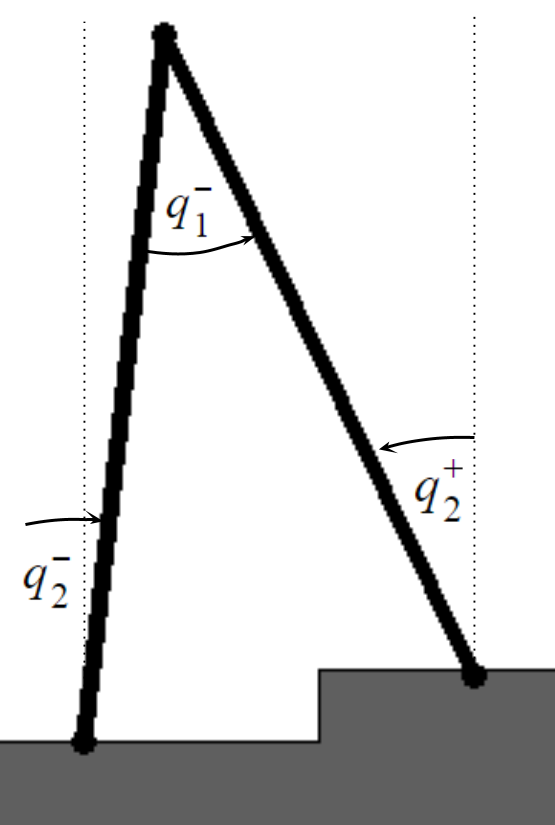
\includegraphics[scale=1]{../images/impact.png}
	\caption{Change of coordinates at impact}
	\label{fig:relabel}
\end{figure}

\subsection{Application of virtual constraints and zero dynamics}
The application of virtual holonomic constraints is a method by which a system's generalised coordinates may be synchronised to a single coordinate, called the \textit{phase variable}, $\theta$. In order for this to be sensible, we assume that $\theta$ is increasing over some interval $[\theta_0, \theta_f]$. Under that assumption, we may construct functions for all of the generalised coordinates of the form:
\begin{equation}
	q_i(t) = \phi\left(\theta(t)\right), ~~ i = 1,2,\ldots,n
\end{equation}
Using trivial differentiation rules, we obtain
\begin{eqnarray}
	\dot{q}_i(t) &=& \frac{\partial\phi\left(\theta(t)\right)}{\partial\theta}\dot{\theta},
						~~i = 1,2,\ldots,n \\
	\ddot{q}_i(t) &=& \frac{\partial^2\phi\left(\theta(t)\right)}{\partial\theta^2}\dot{\theta}^2 +
						\frac{\partial\phi\left(\theta(t)\right)}{\partial\theta}\ddot{\theta},
						~~i = 1,2,\ldots,n
\end{eqnarray}
We define the following vector functions:
\begin{eqnarray}
	\Phi\left(\theta\right) &=& \left[ \phi_1\left(\theta\right), \phi_2\left(\theta\right), \ldots,
	\phi_n\left(\theta\right)\right]^T \\
	\Phi'\left(\theta\right) &=& \left[ \frac{\partial\phi_1\left(\theta\right)}{\partial\theta},
	\frac{\partial\phi_2\left(\theta\right)}{\partial\theta}, \ldots ,
	\frac{\partial\phi_n\left(\theta\right)}{\partial\theta} \right]^T \\
	\Phi''\left(\theta\right) &=& \left[ \frac{\partial^2\phi_1\left(\theta\right)}{\partial\theta^2},
	\frac{\partial^2\phi_2\left(\theta\right)}{\partial\theta^2}, \ldots ,
	\frac{\partial^2\phi_n\left(\theta\right)}{\partial\theta^2} \right]^T
\end{eqnarray} ~\\

Under the assumption perfect regulation of the virtual constraints, thus the above relations holding, we can evaluate the zero dynamics by simple substitution into Equation~\ref{eqn:dynamics}:
\begin{equation}
	M\left(\Phi(\theta)\right)\left[\Phi'(\theta)\ddot{\theta} + \Phi''\dot{\theta}^2\right] + 
	C\left(\Phi(\theta),\Phi'(\theta)\dot{\theta}\right)\Phi'(\theta)\dot{\theta} +
	G\left(\Phi(\theta)\right) = B\left(\Phi(\theta)\right)u_c
\end{equation}
where $u_c$ is the control which achieves perfect regulation of the constraints. This may be rearranged into a more convenient form:
\begin{equation} \label{eqn:zerodyn}
	\alpha(\theta)\ddot{\theta} + \beta(\theta)\dot{\theta}^2 + \gamma(\theta) = 0
\end{equation}
where, if we denote $B^{\perp}(q)$ as a row vector which satisfies $B^{\perp}(q)B(q)u_c = 0$,
\begin{eqnarray}
	\alpha(\theta) &=& B^{\bot}\left(\Phi(\theta)\right)M\left(\Phi(\theta)\right)\Phi'(\theta)\nonumber \\
	\beta(\theta) &=& B^{\bot}\left(\Phi(\theta)\right)\left(M\left(\Phi(\theta)\right)\Phi''(\theta)
		+C\left(\Phi(\theta),\Phi'(\theta)\right)\Phi'(\theta) \right) \nonumber \\
	\gamma(\theta) &=& B^{\bot}\left(\Phi(\theta)\right)G\left(\Phi(\theta)\right)
\end{eqnarray} ~\\
\pagebreak

\subsection{Partial closed-form solutions for velocity and energy}
One of the useful properties of virtual constraints is the ability that they lend the designer of a motion planner to precompute a partial closed-form solution for velocity and energy. The solution is partial in that we obtain an expression for $\dot{\theta}^2$ in terms of $\theta$, rather than $\theta$ in terms of time. Under the assumption that $\theta$ is monotonic, it can be used as a new dependent variable:
\begin{eqnarray}
	\frac{d}{d\theta}\left[\dot{\theta}\left(t(\theta)\right)^2\right] &=& 
	\frac{d}{dt}\frac{dt}{d\theta}\left[\frac{d\theta}{dt}\left(t(\theta)\right)^2\right] \nonumber \\ 
	&=& 2\ddot{\theta}\left(t(\theta)\right)
\end{eqnarray}
Substituting Equation~\ref{eqn:zerodyn} into this expression, we arrive at a first-order ODE in $\dot{\theta}(\theta)^2$:
\begin{equation}\label{eqn:zerodynDE}
	\frac{d}{d\theta}\dot{\theta}(\theta)^2 = -2\frac{\beta(\theta)}{\alpha(\theta)}
		\dot{\theta}(\theta)^2 - 2\frac{\gamma(\theta)}{\alpha(\theta)}
\end{equation}
If we assume, as in \cite{manchester13planning}, that for all $\theta \in [\theta_0, \theta_f]$, we have local instantaneous controllability, i.e. $\alpha(\theta) \neq 0$, then we may solve Equation~\ref{eqn:zerodynDE} numerically over $[\theta_0, \theta_f]$, which yields an affine solution, i.e.
\begin{equation}
	\dot{\theta}(\theta)^2 = \Gamma(\theta, \theta_0)\dot{\theta}_0^2 + \Psi(\theta, \theta_0)
\end{equation}
From this, we may also derive the total mechanical energy of the system. For general systems with dynamics as expressed in Equation~\ref{eqn:dynamics}, the mechanical energy has the form:
\begin{equation}
	H\left(q,\dot{q}\right) = \dot{q}^TM(q)\dot{q} + V(q)
\end{equation}
Under perfectly regulated virtual constraints, this reduces to:
\begin{equation}
	\bar{H}\left(\theta,\dot{\theta}\right) := \Upsilon(\theta)\dot{\theta}^2 + \Xi(\theta)
\end{equation}
where
\begin{eqnarray*}
	\Upsilon(\theta) &=& \Phi'(\theta)^TM\left(\Phi(\theta)\right)\Phi'(\theta) \\
	\Xi(\theta) &=& V\left(\Phi(\theta)\right)
\end{eqnarray*}
Since this is affine in $\dot{\theta}^2$ for a given $\theta$, we may trivially calculate the closed form:
\begin{equation}
	H\left(\theta, \dot{\theta}\right) =
	\Upsilon(\theta)\Gamma\left(\theta,\theta_0\right)\dot{\theta}_0^2 +
	\Upsilon(\theta)\Psi\left(\theta,\theta_0\right) + \Xi(\theta)
\end{equation}
\pagebreak

\section{B{\'e}zier curves as virtual constraints}
Bézier curves provide a way to produce families of curves for particular start and end heights and are sparsely identified by only $n+1$ points, where $n$ is the degree of the curve. These points provide an intuitive way of defining the curve, in contrast with polynomial coefficients.
\par

Theoretically, these curves need only be defined from the start to the endpoint of the continuous-phase which they specify. However, since the curve provides a virtual constraint to be enforced by a controller, it is necessary to define the curve over the full range of possible motion, here considered to be $\theta_1 \in \left[0, \pi\right]$, else it is possible for the walker to enter a region where the control signal is undefined. If we assume that the overshoot past the desired endpoint is small, then the shape of the curve should be flat outside the defined region. That is, when we leave the target region, we wish to set $\theta_2$ to the closest defined $\theta_2$. \\ \par

For the compass-gait walker, a general Bézier curve is defined by the following parametric equation.
\begin{equation}
	\begin{bmatrix}
		\theta_1 \\ \theta_2
	\end{bmatrix}
	=
	\sum_{i=0}^{n}\binom{n}{i}\left(1-t\right)^{n-i}t^i
	\begin{bmatrix}
		\theta_{1_i} \\ \theta_{2_i}
	\end{bmatrix} \label{eqn:genBez}
\end{equation}
Since this equation is not monotonic in $\theta_1$, it is not a convenient expression. Therefore, we build families of Bézier curves with the following formulation:
\begin{eqnarray}
	t &=& \frac{\theta_1 - \theta_{1_0}}{\theta_{1_n} - \theta_{1_0}} \\
	\theta_2 &=& \sum_{i=0}^{n}\binom{n}{i}\left(1-t\right)^{n-i}t^i\theta_{2_i}
\end{eqnarray}
This is expressible explicitly as
\begin{equation}
	\theta_2 = \frac{1}{\left(\theta_{1_n} - \theta_{1_0}\right)^n}\sum_{i=0}^{n}\binom{n}{i}
		\left(\theta_{1_n} - \theta_1\right)^{n-i}
		\left(\theta_1 - \theta_{1_0}\right)^i\theta_{2_i} \label{eqn:expBez}
\end{equation}
This formulation removes our ability to arbitrarily define the control points $\left(\theta_{1_i}, \theta_{2_i}\right)$, other than the endpoints. That is, this formulation produces curves of the form given in Equation~\ref{eqn:genBez} with
\begin{equation}
	\theta_{1_i} = \frac{i}{n}\left(\theta_{1_n}-\theta_{1_0}\right) + \theta_{1_0} ~~
	\forall ~~ i \in \left[1,~n-1\right]
\end{equation}

Since we can only define one of the two variables in each control point, to yield arbitrary curves of order $n$, before achievable with $n - 1$ free control points (i.e. non-endpoint control points), now requires $2n - 2$ such points. Since it is desirable to have the ability to set the gradient of approach to the control points independently of the shape of the polynomial (achievable using a general cubic Bézier curve) we use a quintic curve in the new formulation. This requires six control points.
\clearpage

\chapter{Virtual Constraint Library}
\setcounter{figure}{0}\setcounter{equation}{0}\setcounter{table}{0}
\section{Requirements for a useful library}
The utility of a library of motion primitives is dependent on the suitability of the gaits which may be produced by the composition of elements of the library to the terrain over which the robot must locomote. Furthermore, in order for an algorithm which chooses between the constraints within the library to realise the benefits of motion planning with primitives as discussed in Section \ref{sec:primplanning}, the constraints must be stored in a manner which enables the algorithm to intelligently discriminate between them. To comply with these conditions, the virtual constraint library must satisfy requirements which may be broadly classed as \textit{physical} and \textit{algorithmic}.

\subsection{Physical requirements}
Feasible walking (single constraint)
- Collision-free paths
- Dynamic feasibility -- not falling back: Equation \ref{eqn:critvel}

Physical realisability (single constraint)
- torque limits
- Friction cone

Library requirements
- Sufficient coverage of motions
- Compatibility between constraints (invariance)

\subsection{Algorithmic requirements}
- Psi, Gamma at useful points
- Identification of start and end configuration
- Means for testing or ensuring that the physical requirements are satisfied
- Some kind of ordering

\subsection{Practical considerations}
A library satisfying the above requirements is sufficient to ensure that walking motions are in principle able to be generated for the set of terrains over the applicable set of terrains, however there are additional considerations for a system to be useful in practice.

- Optimality
- Degree of constraints
- Uncertainty
- Space vs on-line computation efficiency
- Number of constraints in library - Too many and search becomes cumbersome/library is wasteful, too few and the library does not present adequate coverage.

\section{Data stored per constraint}
\input{4VirtConstLib/2Data}

\section{Graphical interface for constraint design}
When attempting to design virtual constraints for a robot, even if the goal is to generate them automatically, it is instructive and useful to have a means of examining the properties of virtual constraints and their associated partial solutions. A graphical user interface (GUI) is a particularly efficient and intuitive tool to this end. The GUI created for investigation of virtual constraints has four main features; observing the curve in Bézier space and the corresponding path in Cartesian space, investigating the shape of the partial solution given a particular virtual constraint, facilitating the slicing of the Bézier coefficient decision variable space to confirm convexity and displaying the nominal torque given a VC and an initial velocity. The GUI is also able to display the optimal coefficients based upon some start and end configuration (see Section \ref{sec:singleVCopt}) along with the graph of $\Gamma(\theta^c), \Psi(\theta^c)$ in order to investigate ordering methods (see Section \ref{sec:orderings}).

The interface is implemented in MATLAB and saves any chosen virtual constraints to the workspace. The GUI is flexible in that it is usable for any planar bipedal robot model. Figure \ref{fig:guiCG} demonstrates the typical display of the interface for the compass-gait (2-link). The software may prove useful for others to investigate the properties of virtual constraints and is therefore made freely available online, along with the other code used to generate the results for this thesis, at github.com/swardrop/virtualconstraints.

\begin{figure}
	\centering
	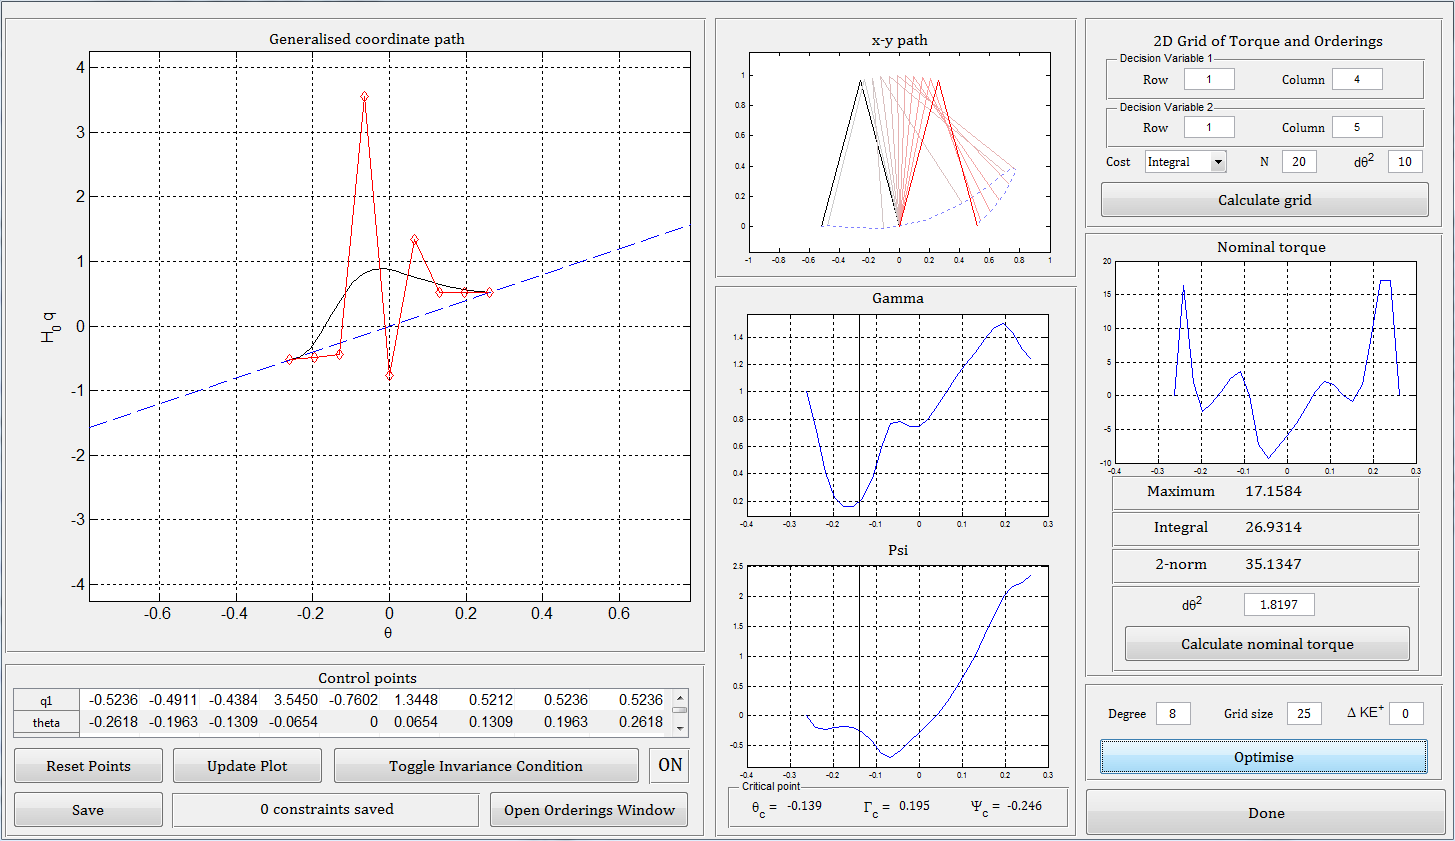
\includegraphics[width=0.9\linewidth]{4VirtConstLib/guiVC.png}
	\caption{Graphical interface for virtual constraint design showing compass-gait model}
	\label{fig:guiCG}
\end{figure}

\section{Single constraint optimisation}
\subsection{Motivation for optimisation approach}
Most approaches to designing Bézier polynomial-based virtual constraints for a bipedal robot can be classed in one of three categories; \textit{manual design}, \textit{sampling} or \textit{optimisation}. Manual design involves a human operator producing the control points directly. Sampling is the utilisation of some method of choosing coefficients in an attempt to span the configuration space, either by random selection or gridding. Optimisation approaches choose coefficients which minimise some cost function under particular constraints.

Manual design approaches are not favourable since they are expensive and inefficient in comparison to automatic generation of virtual constraints. Sampling methods, while much faster at generating a single virtual constraint than manual generation, suffer from the \textit{curse of dimensionality}. That is, in order for a sampling method to produce the same density of coverage, the number of samples required increases exponentially with the number of dimensions. Using a brute-force sampling approach produces many redundant primitives which exhibit similar net changes in the mechanical energy of the walker and paths of the end of the swing leg. It is also difficult to ensure that the conditions for feasible walking are met using pure sampling methods.

The redundancy inherent in the sampling approach increases the the memory required to store the virtual constraint library and the computational requirements of both its generation and use in real time. An optimisation approach attempts to find the best virtual constraint subject to particular requirements, e.g. beginning and final conditions. Therefore, the utility of single virtual constraint optimisation is to avoid the large amount of redundancy involved in the sampling approach and to enable the enforcement of feasible walking conditions. Clearly, single VC optimisation is itself not sufficient to produce a library of primitives; see Section \ref{sec:lib}.

\subsection{Definition of optimality}
As with most physical systems, there are competing definitions of optimality in the case walking robots; {\color{red}<insert literature references to competing definitions>}.

The definition of optimality chosen for the purposes of producing the virtual constraint library is as follows:
\emph{The optimal virtual constraint for a given start and end configuration and kinetic energy gain or loss is the one which requires the minimum input energy to maintain.}

We note that the relationship between torque and electrical energy in conventional DC motors is typically approximated by the following equation:
\begin{equation} \label{eqn:motorenergy}
	E(t) \approx \int\limits_0^t u(s)^2 ~ ds
\end{equation}

However, since the partial solution of the zero dynamics is in terms of $\theta$ rather than time, this is not a convenient cost function. Therefore, we assume that $\theta$ progresses reasonably steadily on the interval $[\theta^+,~\theta^-]$ and thus the cost function
\begin{equation}
	J_\alpha = \int\limits_{\theta^+}^{\theta^-} \left\lVert u_\alpha(\theta) \right\rVert_2^2 ~ d\theta
\end{equation}
approximates Equation \ref{eqn:motorenergy} evaluated over the virtual constraint. Note that the L2-norm is included to encapsulate the contribution of multiple torques, since in all but the simplest walking robots, there is more than one actuated joint.

\subsection{Validity of convex optimisation approach}
The decision variables for the purpose of optimisation are the Bézier coefficients $\alpha$. Since the formulation of the cost function $J$ is not linear or quadratic in these decision variables, the optimisation problem becomes more complex; see Section \ref{sec:nonlinopt}. Linear and quadratic techniques are not immediately applicable to the nonlinear case, leaving two alternatives; gridding approaches and nonlinear programming. Gridding approaches in optimisation are subject to the same limitations described above; indeed, if the advantage of optimisation is to avoid using gridding, then such an approach is clearly a poor choice. However, nonlinear programming will only produce reasonable results under certain conditions.

It is not possible to determine \textit{a priori} that an optimisation is well-formed, that is, will result in a valid solution. Furthermore, for nonlinear optimisation to produce favourable results, the cost function must be convex or near-convex close to the initial estimate. It is therefore of significant interest to determine how close the cost function is to being convex. For the two-link compass gait walker, it is possible to produce such a verification, since we can formulate an optimisation with only two decision variable,s which is easily visualised. In Figure \ref{fig:cggridtorque}, we see that gridding the two decision variables produces a surface that appears to be well-behaved and convex. It is reasonable to suggest that this is generalisable to higher degree constraints with more decision variables for the compass-gait robot.

\begin{figure}
	\centering
	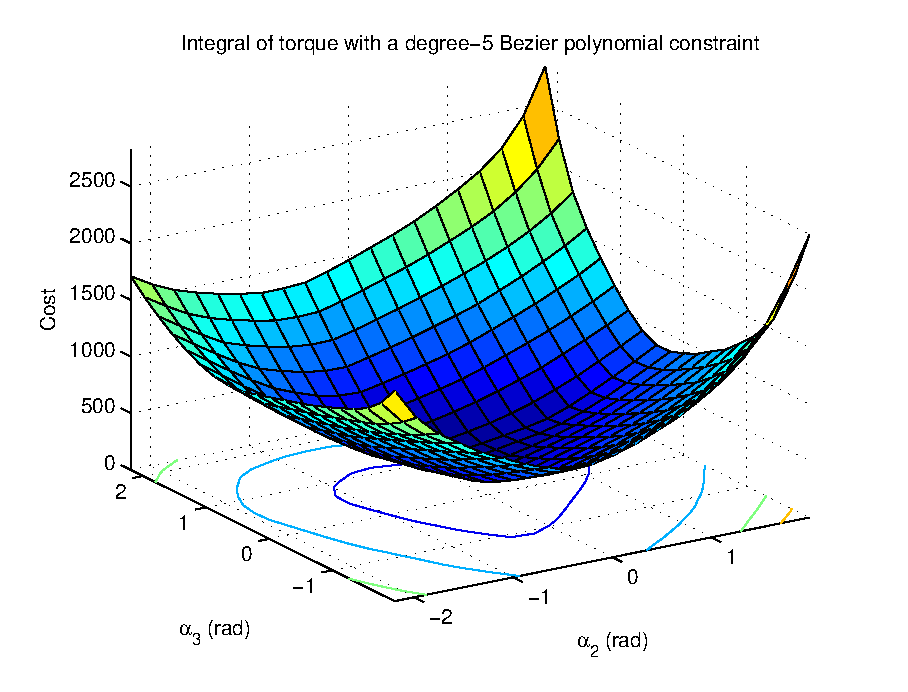
\includegraphics[width=0.8\linewidth]{4VirtConstLib/CGgrid.eps}
	\caption{Cost function of a two decision variable compass-gait optimisation}
	\label{fig:cggridtorque}
\end{figure}

In the case of higher-DOF walking models, it becomes more difficult to confirm near-convexity or even that the cost function is well-behaved. Taking slices, where we choose two decision variables over which to grid and fix all others, allows us to develop some intuition, see Figure \ref{fig:5lslice1} and \ref{fig:5lslice2}. We note that in these slices, the cost function again appears to be well-behaved and near-convex. On the basis of this evidence, it appears to be reasonable to assume that the convex optimisation approach will produce valid near-optimal results.

\subsection{Optimisation method}
\subsubsection{Decision variables and constraints}
While the objective of single constraint optimisation is to produce an optimum VC independent of any other virtual constraints in the library, it is important to formulate the optimisation problem in a manner which enables a useful library to be produced. The motion primitive library is intended to contain VCs which span the configuration space of the robot's natural walking as well as including a range of mechanical energy additions and subtractions to facilitate walking over uneven terrain. Therefore, it seems clear that each single constraint optimisation should be formulated subject to constraints on the start and end configurations of the footstep, along with a prescribed energy gain or loss. In addition, it is necessary to specify the ground height applicable to the virtual constraint, since a feasible step cannot intersect with the ground between the start and end conditions.

Since the potential energy change is prescribed by the start and end conditions, it is convenient to formulate the optimisation using kinetic, rather than total mechanical, energy. The change in kinetic energy $\Delta$KE from one footstep to the next could be calculated with respect to numerous reference points. A simple and obvious choice is to define $\Delta$KE as the change in kinetic energy from $\theta_\alpha^+ \rightarrow \theta_\beta^+$, with $\beta$ being the constraint which follows $\alpha$.

The ground height at a horizontal displacement $x$ from the end of the stance leg is encoded in the scalar function $\sigma(x)$. For the purposes of analysing a virtual constraint, the ground height is pertinent only when considering the end of the swing leg, thus we may produce a more convenient representation $\sigma(\theta)=\sigma(p_h(\theta))$. The ground height places the following nonlinear constraints on the optimisation:
\begin{equation} \label{eqn:groundheight}
	p_v(\theta) \left\{
	\begin{array}{lcr}
		= \sigma(\theta) &:& \theta \in \{\theta^+, \theta^-\} \\
		> \sigma(\theta) &~& \mathrm{otherwise}
	\end{array} \right.
\end{equation}

Recall from Section \ref{sec:bezconstraints} that in order to be physically realisable, a VC must satisfy several conditions. The \textit{invariance conditions}, \ref{item:configinvariance} and \ref{item:velinvariance}, place restrictions on the admissibility of a primitive on the basis of the VC which preceded it. The first condition is not of great concern in the construction of a single primitive, since the responsibility of ensuring coverage of start and final configurations is deferred to the library generation. However, it is important to consider the latter condition when generating a single constraint; in order for the library to be useful, any VC which matches the prior primitive through the impact map should be a valid choice of successor. This implies that the slope of all constraints at the end point for any given final configuration ought to be identical. A reasonable choice to satisfy this condition is to enforce that the final slope must be zero for all constraints. This has the additional advantage of making the constraints more robust to errors in ground height perception.

When formulating an optimisation, it is advantageous to minimise the number of decision variables, if all else is considered static, since this reduces the evaluation time. This is particularly true for variables which are subject to constraints. It is notable that fixing the start and end configuration of the constraint along with enforcing zero slope at the final configuration fixes the four outermost columns of $\alpha$. As such, we consider these fixed and exclude them as decision variables. The optimisation variables therefore take the form given in Table \ref{tab:optDecVars}. Note that the conditions in Section \ref{sec:bezconstraints} along with the equality constraint in Equation \ref{eqn:groundheight} are all concerned with those four outermost columns of $\alpha$, therefore in the single VC optimisation, these conditions are not applicable.

\begin{table}
	\centering
	\begin{tabular}{c | c | c | c}
		            Variable             & Generated                     & Decision Variable & Opt constraint \\ \hline
		   $\theta^+$ and $\theta^-$     & From start/end condition      & No                & No             \\
		   $\alpha_0$ and $\alpha_N$     & From start/end condition      & No                & No             \\
		         $\alpha_{N-1}$          & Set to $\alpha_N$             & No                & No             \\
		           $\alpha_1$            & From \ref{item:velinvariance} & No                & No             \\
		$\alpha_2, \ldots, \alpha_{N-2}$ & Optimisation                  & \textbf{Yes}      & No             \\
		           $\Delta$KE            & Supplied                      & No                & \textbf{Yes}   \\
		           $\sigma(x)$             & Supplied                      & No                & \textbf{Yes}
	\end{tabular}
	\caption{Variables involved in the single VC optimisation}
	\label{tab:optDecVars}
\end{table}

\subsubsection{Nominal initial velocity}
The torque required to maintain a virtual constraint is not only dependent on the configuration path, but also the velocity. VCs prescribe the configuration path and constrain the velocity to be a function of the initial phase variable velocity. As a result, the torque required to maintain a virtual constraint is a function of the initial velocity. In addition, $\Delta$KE is affine in the square of the initial phase variable velocity. It is therefore necessary to formulate a \textit{nominal initial velocity}, $\dot{\theta}^*$. We assume that in practice, the constraint will be chosen with initial velocities close to $\dot{\theta}^*$ and should therefore be near-optimal. Under that assumption, the change in kinetic energy should be close to the prescribed $\Delta$KE, however this is less important since the fixing of $\Delta$KE is in service of producing a rich library.

Choosing a nominal velocity for each constraint is non-trivial. It should be noted that the choice of nominal velocity significantly influences the optimisation. Fixing $\dot{\theta}^*$ is not appropriate, each virtual constraint may differ in the minimum velocity required to complete the motion. It seems necessary to treat the constraints separately based upon the desired $\Delta$KE.

For \textbf{energy-additive constraints}, for which $\Delta$KE $>0$, the key issue of importance is that the virtual constraint itself is feasible, since the next primitive will have additional kinetic energy. Therefore, we set the initial velocity such that $\dot{\theta}^* = \lambda\dot{\theta}^+_c$, where $\lambda$ is some fixed ``factor of safety'':
\begin{equation} \label{eqn:energyadditive}
\dot{\theta}_{\Delta\mathrm{KE}^+}^{*^2} = -\lambda^2\frac{ \Psi(\theta_c)}{ \Gamma(\theta_c)}
\end{equation}

For \textbf{energy-subtractive constraints}, for which $\Delta$KE $<0$, assuming that the robot should never come to a stop or fall back, the energy reduction should result in further constraints being feasible. In order to avoid using any data external to the constraint, we use the value of $\dot{\theta}^+_c$ associated with the same VC. The post impact velocity is calculable with $\Delta_{\dot{\theta}}$ as defined in Equation \ref{eqn:Delthd}:
\begin{subequations}
	\begin{align}
	\left(\dot{\theta}^-\right)^2 &= \Gamma(\theta^-)\dot{\theta}^{*^2} + \Psi(\theta^-) \\
	\dot{\theta}^+ &= c\Delta_{\dot{\theta}}\dot{\theta}^-
	\end{align}
\end{subequations}
Equating $\dot{\theta}^+$ with $\lambda\dot{\theta}^+_c$, where $\lambda$ is the same factor of safety as in Equation \ref{eqn:energyadditive}:
\begin{equation}
	\dot{\theta}_{\Delta\mathrm{KE}^-}^{*^2} = \frac{(c\Delta_{\dot{\theta}})^{-2}\left(-\lambda^2\frac{ \Psi(\theta_c)}{ \Gamma(\theta_c)}\right) - \Psi(\theta^-)} {\Gamma(\theta^-)}
\end{equation}

\textbf{Energy-neutral constraints}, for which $\Delta$KE $=0$, result in $\dot{\theta}^+ = \dot{\theta}^*$. That is, if the constraint is entered into with an initial velocity equal to the nominal velocity, the post-impact velocity will equal the initial velocity. For these constraints, so long as the ground is identical through the footsteps, choosing the same footstep repeatedly will result in nominal periodic motion. This should not be confused with the stable limit cycles of \cite{grizzle2001asymptotically, franken2008analysis}, since there is no guarantee of stability; a small deviation may cause the walker to diverge or to converge to some nearby stable limit cycle. The key issue here is that, since at the nominal velocity the post-impact velocity is identical to the initial velocity, the two formulations are equivalent. The simplicity of Equation \ref{eqn:energyadditive} is preferred.

\subsection{Implementation}
The single VC implementation is achieved using MATLAB's constrained nonlinear programming function \mcode{fmincon}. This uses an interior point method to seek local minima in the cost function subject to the given constraints. For each set of test values for the decision variables, the partial solution ($\Gamma(\theta)$ and $\Psi(\theta)$) is evaluated by producing a grid of $\theta$ values in $[\theta^+, \theta^-]$. The cost is calculated using trapezoidal integration on the resulting torque values. Since $\Delta$KE also relies upon the partial solution, it is held persistently in a helper function and only recalculated upon differing decision variables, to avoid inefficient recalculation.

$\sigma(x)$ is defined by specifying the ground height at individual points. From this, the ground level over all $x$ is determined by a zero-order hold. The ground constraint is enforced by taking relatively sparse samples from $\theta^+$ to $\theta^-$ and testing for each sample that $p_v(\theta)>\sigma(\theta)$. A natural choice of samples is at each Bézier control point, such that the sampling of the ground is dependent on the degree of the polynomial. It is reasonable to test only several points along the trajectory on the assumption that the ground height changes at relatively few points over one footstep and that the swing leg traces a smooth arc between its start and end points. The second assumption is valid for all physical robots. The first is able to be justified by the design of the library generation.

The optimisation is not subjected to any additional bounds other than the $\Delta$KE and $\sigma(x)$ constraints. This is due to the well-behaved nature of the problem; large deviations always cost more in terms of input torque than small ones. It therefore makes little sense to arbitrarily constrain the decision variables. In the case of the compass-gait robot, due to its morphological simplicity, the $\sigma(x)$ constraint is not applied. Indeed, it is not possible for the compass-gait robot to complete walking motion on flat ground without scuffing its swing leg if no means are provided to shorten it.

The \mcode{optimiseConstraint} function takes as arguments the start and end configurations of the constraint, the desired change in kinetic energy, the ground definition $\sigma(x)$ and the degree of the desired Bézier polynomial. It returns the start and end values of the phase variable $\theta^+$, $\theta^-$ and the Bézier coefficients $\alpha$. These are sufficient to define the virtual holonomic constraint, however, for convenience, it also returns the calculated values of the partial solution at $\theta^+$, $\theta^-$ and $\theta_c$.

\section{Library generation}
Library generation is the process of creating of a large set of primitives $P$, each of which define a trajectory $\Phi(\theta^+) \to \Phi(\theta^-)$, where $\Phi(\theta^+), \Phi(\theta^-) \in \tilde{Q}$, the set of all impact configurations. The library is intended to be structured such that efficient on-line use is enabled. Minimising off-line computation time is a secondary concern.

\subsection{Acceptable coverage}
As motivated in the previous section, a useful library of motion primitives for walking over uneven terrain requires coverage over the start and final configurations of the robot along with a range of kinetic energy additions and subtractions. Depending on the unevenness of the terrain, a diverse range of paths of the end of the swing leg may also be required. All generated constraints should be admissible and usable to avoid wasted memory and computation time.

While it is clear that some density of coverage is required, it is not immediately obvious what constitutes sufficiency. It is advantageous to avoid over-populating the library in order to speed up its generation and real-time use and reduce the memory requirements. However, advantages in computation time are meaningless if the library is insufficient for its purpose. As a result, methods for defining acceptable coverage of the dimensions of this optimisation are required.

\subsubsection{Start and end configurations}
It is essential that the library is designed such that final configurations of virtual constraints match initial configurations of other constraints through the impact map. A primitive is not useful if there are no primitives which can succeed it. Other than a detailed study of the terrain on which the robot is intended to be used, there is no good means for deciding on sets of configurations which should be reachable through a single constraint from a given configuration, therefore it seems necessary to generate a set of virtual constraints linking each pair in $\tilde{Q}\times\tilde{Q}$. This provides further motivation to avoid specifying more impact configurations than necessary, since the number of virtual constraints in the library $\lvert P \rvert \propto \lvert\tilde{Q}\rvert^2$.

The most important consideration for impact configuration coverage is to ensure that there is a relatively fine grid of vertical displacements $p_v(\theta^-)$ for a given horizontal displacement to allow for the traversal of the robot over unpredictable terrain. The resolution and bounds of this grid should chosen be such that the intended terrain is properly discretised; large gaps between the upper/lower bounds and the maximum displacement of the expected terrain should be avoided. Certainly, the upper and lower bounds should not exceed the capability of the robot. Furthermore, the resolution should be comparable in size to the combined error in the robot's perception of the terrain and the closeness to which the controller can regulate a trajectory. As is evident from these requirements, the best choice of grid for height values depends on the terrain and robot for which the library is being designed. We denote the number of unique step heights $n_y$.

It is much less important to have a dense grid of horizontal displacements. Indeed, dynamic walking over uneven terrain in most instances achievable with a fixed step length. This fact forms the basis of much of the previous work using feedback-stabilised periodic gaits to enable locomotion over relatively uneven terrain \cite{bigdog?}. Having a set of step lengths is advantageous in that it enables for intelligent foot placement. Denote the number of unique step lengths $n_x$.

Other than in the case of the compass-gait robot, the step length and height are not sufficient to specify the final configuration of the robot. It is therefore necessary to perform inverse kinematics to generate joint angles. In the general case, there are infinitely many combinations of joint angles which can produce the final configuration for a particular step length and height. There is no general method for producing the best configuration; it depends on the robot's mechanical design and the desired gait. While not strictly necessary for terrain scalability, the energy efficiency of planned trajectories can be improved by having multiple configurations of joints per step length and height from which to choose. Let us denote the number of these configurations $n_q$.

The cardinality of the set of all impact configurations is trivially evaluable:
\begin{equation} \label{eqn:numimpactconfs}
\lvert\tilde{Q}\rvert = n_xn_yn_q
\end{equation}
We note that while $n_q$ must be fairly large to enable walking over uneven terrain, $n_x$ and $n_q$ are useful only to provide additional control and should be kept small. Under Equation \ref{eqn:numimpactconfs}, $\lvert P \rvert \propto \lvert\tilde{Q}\rvert^2 \implies \lvert P \rvert \propto n_x^2 ~~\wedge~~ \lvert P \rvert \propto n_q^2$.

\subsubsection{Inter-step kinetic energy changes}
The only method of velocity control available to the motion planner is to chose constraints which add, maintain or reduce the kinetic energy of the walker. It is therefore important to produce, for each pair of step length and height, a range of kinetic energy mutations. For simplicity, we produce a set of kinetic energy additions and subtractions $\tilde{K}$, where $\lvert\tilde{K}\rvert = n_k$. For each set of initial and final configurations $q^+,q^- \in \tilde{Q}$, we produce the $n_k$ unique trajectories $q^+ \to q^-$ with $\Delta$KE $\in \tilde{K}$.

For a given robot, it may be possible to define a particular range of $\Delta$KE values on the basis of the initial and final configuration. For instance, since a step-up trajectory converts kinetic into potential energy, constraints which add the maximum kinetic energy may not ever be chosen by the motion planning algorithm. Such reasoning is difficult to properly justify in general and as such has not been pursued in this thesis work. Even if such reasoning is used, it is still likely best to produce $n_k$ paths.

We need not be as strict on keeping $n_k$ small, since $\lvert P \rvert \propto n_k$ rather than $n_k^2$, however since velocity control is able to be executed over multiple footsteps, the precision and variety of $\Delta$KE over a single footstep is not critical. Therefore in the interest of keeping the library manageable, $n_k$ should be kept to a moderate size.

Note that while the initial and final configurations are important data for a virtual constraint, the $\Delta$KE should not be stored. As discussed previously, the change in kinetic energy is dependent on the initial velocity of the constraint. Furthermore, its calculation requires very little computation due to the affine form of the partial solution.

\subsubsection{Ground configurations}
It is important to consider the likely shape of the ground for constraints with particular step lengths and heights. For the off-line generation of virtual constraints, it is best to be somewhat conservative in specifying where the ground level changes. Consider Figure \ref{fig:stepup}; the terrain steps up at a horizontal displacement significantly smaller than $p_h(\theta^-)$. It is reasonable to expect that this is representative of the typical use case of a step-up virtual constraint. It is not necessary to optimise numerous primitives with all else fixed, but with varied ground configurations; if the terrain profile for the purposes of each single VC optimisation is conservatively defined, the ground configuration is indirectly sampled by producing constraints with varying initial and final configurations.

\begin{figure}
	\centering
	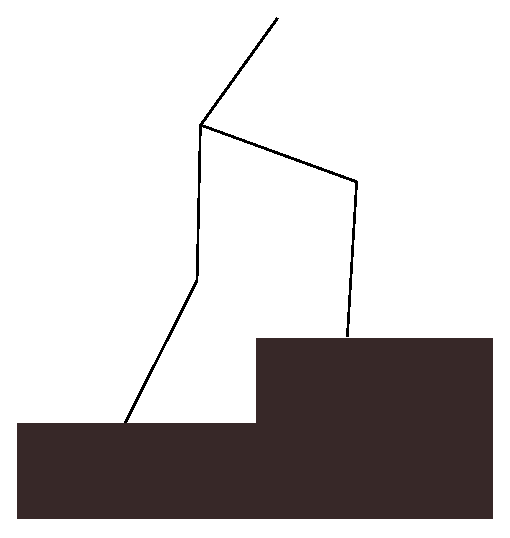
\includegraphics[width=0.5\linewidth]{4VirtConstLib/stepup.eps}
	\caption{Example step-up showing possible terrain profile}
	\label{fig:stepup}
\end{figure}

\subsection{Ordering sets of constraints} \label{sec:orderings}
As discussed in Section \ref{sec:primplanning}, planning with primitives is made much more efficient if there is an ordering of primitives, since this facilitates a binary search, reducing the worst-case search time from $O(n)$ to $O(\log n)$. Ordering on the basis of $\Gamma(\theta^\bullet)$ and $\Psi(\theta^\bullet)$

\subsection{Library structure}
The structure of the library is a critical issue in determining the running time of the planning algorithm. It is important that constraints with certain properties can be found efficiently and that traversal through the library is straightforward. The library of motion primitives is structured similarly to that described in \cite{manchester13planning}.

The library is built using a hierarchical (forest) structure with each of the impact configurations in $\tilde{Q}$ at the top. Consider this the initial configuration of the robot. Connected to each root node are $n_x$ nodes representing a particular step length $p_h(\theta^-)$. To each of these nodes are connected $n_y$ edges, encoding the grid of step heights $p_v(\theta^-)$. At each of the nodes reachable from these edges, we have an encoded step length and height. This is important since there is only one height for a given length which is applicable based on the terrain.

Each of these nodes is connected to $n_q$ leaf nodes which specify the complete final configuration $q(\theta^-)$ of the robot. For each final configuration, there are $n_k$ applicable trajectories $q^+ \to q^-$, specified by Bézier coefficients as discussed in Section \ref{sec:bezconstraints}. These paths are able to be sorted based upon the ordering method introduced in Section \ref{sec:orderings}.

The library is therefore conducive to an efficient search from a particular initial configuration $q^+$ to a trajectory $q^+ \to q^-$ on the basis of first matching step heights to the terrain at given step lengths, then searching through only the applicable constraints for a desired velocity or kinetic energy. Note that since the primitives are ordered, this search is completed in $\mathcal{O}(n_x\log(n_qn_k))$ time. This is clearly preferable to the $\mathcal{O}(n_xn_yn_qn_k)$ time of a search through an unstructured array.

\begin{figure}
	\centering
	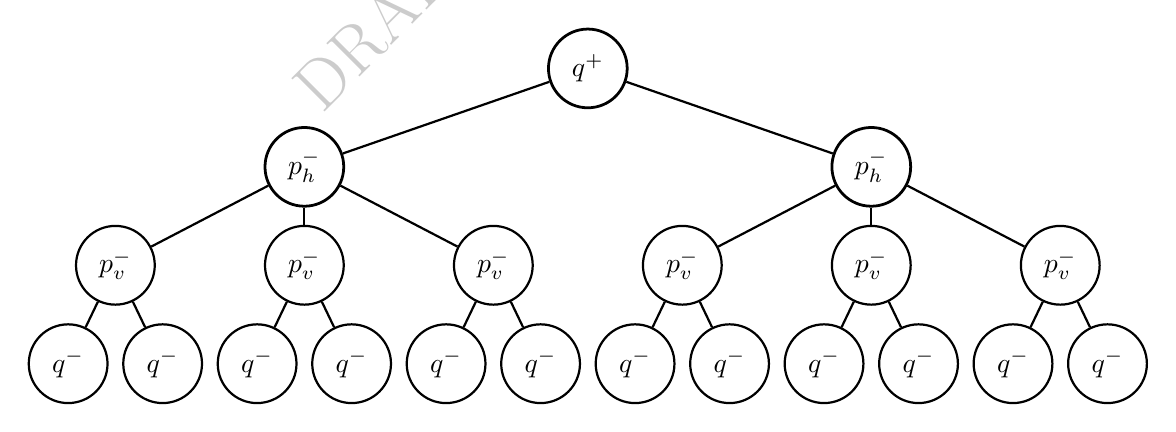
\begin{tikzpicture}[
	scale = 1, transform shape, thick,
	every node/.style = {draw, circle, minimum size = 10mm},
	grow = down,  % alignment of characters
	level 1/.style = {sibling distance=7.2cm},
	level 2/.style = {sibling distance=2.4cm}, 
	level 3/.style = {sibling distance=1.2cm}, 
	level distance = 1.25cm
	]
	\node[shape = circle, draw, line width = 1pt,
	minimum size = 10mm, inner sep = 0mm] {$q^+$} 
	child { node[shape = circle, draw, line width = 1pt,
		minimum size = 10mm, inner sep = 0mm] (x1) {$p_h^-$}
		child {   node [] (A) {$p_v^-$}
			child { node [] (B) {$q^-$}}
			child { node [] (C) {$q^-$}}
		}
		child {   node [] (D) {$p_v^-$}
			child { node [] (E) {$q^-$}}
			child { node [] (F) {$q^-$}}
		}
		child {   node [] (D1) {$p_v^-$}
			child { node [] (E1) {$q^-$}}
			child { node [] (F1) {$q^-$}}
		}}
	child { node[shape = circle, draw, line width = 1pt,
		minimum size = 10mm, inner sep = 0mm] (x2) {$p_h^-$}
		child {   node [] (A1) {$p_v^-$}
			child { node [] (B1) {$q^-$}}
			child { node [] (C1) {$q^-$}}
		}
		child {   node [] (D1) {$p_v^-$}
			child { node [] (E1) {$q^-$}}
			child { node [] (F1) {$q^-$}}
		}
		child {   node [] (D3) {$p_v^-$}
			child { node [] (E3) {$q^-$}}
			child { node [] (F3) {$q^-$}}
		}
	};
	\end{tikzpicture}
	\caption[Virtual constraint library structure]{Virtual constraint library structure. Note that only  one initial condition $q^+\in\tilde{Q}$ is pictured. The library contains many repetitions of this structure.}
\end{figure}
\subsection{Library generation implementation}

\clearpage

\chapter{Algorithm Design}
\setcounter{figure}{0}\setcounter{equation}{0}\setcounter{table}{0}
\section{Requirements for a practical planner}
The role of the motion planner is to select a sequence of primitives which are dynamically feasible and enable the robot to traverse across the terrain between its start and end point. In general, ensuring dynamic feasibility of a trajectory for an underactuated system requires complicated computations, solving multivariate nonlinear differential equations. Fortunately, as discussed in Section \ref{sec:hzd}, using virtual constraints as motion primitives simplifies the zero dynamics to a function of a single variable and simplifies evaluating dynamic feasibility to a trivial verification of the initial velocity exceeding a lower limit.

As a result, the practical requirements on the motion planner are to ensure that each choice of primitive is performed such that both that primitive and another which follows and matches the terrain is able to be completed. For a useful robot, the initial and final conditions should be at some statically stable resting configuration, however for the purposes of this body of work, it is assumed that the robot begins with some non-zero velocity conducive to dynamically stable walking and need never come to rest. That is, the motion planner is not concerned with the practical considerations of starting or ceasing motion.

Aside from the essential functional requirement of choosing dynamically feasible sequences of primitives, the performance requirements on the planner are quite stringent. Since the objective of this approach is to allow for real-time reactive planning of walking, it is essential that the planner is capable of producing a planned sequence of footsteps in a time span shorter than that taken by the shortest footstep. Note that it is likely that a physical implementation would be in a low-power embedded system which executes software alongside the planner. Clearly, computational efficiency is a large priority for the planning algorithm. This is no surprise, since the motivation for using the virtual constraints method itself is largely in service of reducing on-line computational requirements.

\section{Execution context}
The motion planning algorithm is executed using an iterative receding finite horizon approach. This means that the planner produces a dynamically feasible sequence of some set number of footsteps ahead of the current position, but re-evaluates the sequence significantly earlier than the end-point. This can be considered a form of model-predictive control \cite{camacho2013model}.

For convenience of implementation, we may assume that the planner completes an execution once per footstep. In principle, without disturbances, the planner could execute in a purely feed-forward manner. That is, the path would only be recalculated once the robot reached the endpoint of the previously calculated sequence of primitives. In practice, this is typically not possible; the dynamical model, particularly about impacts, is not a full realisation of the physical system. In addition, it is a very useful property for a planner to produce self-correcting trajectories. Indeed, the planning need not be limited to a single evaluation per footstep. However, assuming disturbances are significantly managed by the controller, it should be sufficient.

The planner requires the initial state (configuration and velocity) $q,\dot{q}$ of the robot, along with an accurate map of the terrain ahead. The necessity of state sensing is unavoidable, both in the planning and control of the robot. However, the sensing requirements of underactuated walkers should not be intensive due to deferring control of the state evolution to the zero dynamics \cite{collins2005efficient}. The practice of using sensor data to build a terrain map is well-studied, with advancements in the field moving well beyond simple shape mapping to classification \cite{herbert1989terrain, triebel2006multi, brooks2007self}. The algorithm proposed is largely independent of the method used to build the map, whether by prior mapping or real-time scanning, so long as the range of known terrain extends far enough to allow for the chosen number of footsteps ahead to be planned.

\section{Greedy best-first search algorithm}
Manchester \& Umenberger \cite{manchester13planning} present a greedy Best-First Search algorithm capable of producing a dynamically feasible sequence of $k$ motion primitives. This algorithm, somewhat modified in order to suit the generated library from Chapter \ref{chap:vclib}, is presented in Algorithm \ref{alg:bestfirstsearch}.

\begin{algorithm}
	\begin{algorithmic}[1]
		\Function {BestFirstSearch}{$q,\dot{q},\sigma(x),k$}
		\EndFunction
		\Function {AddNode}{$q,\dot{q},\sigma(x),k$}
		\EndFunction
	\end{algorithmic}
	\caption{Best-first search planning algorithm}
	\label{alg:bestfirstsearch}
\end{algorithm}

The best-first search is dependent upon a worker function \textsc{SearchLibrary}($q^+,s_l,s_h,a$) which returns the primitive which has the smallest $\dot{\theta}(\theta^c) \geq a$ in the set of virtual constraints which match the given initial configuration, step length and step height. Note that for the first primitive, on {\color{blue} L<>}, this function searches through the roots of the trees in the library for $q^+$, but subsequent calls to this function include a pointer to the applicable tree in the library.

\section[Energy-based heuristic]{Improvements using an energy-based heuristic}
Using heuristic methods can direct the decision tree traversal to avoid primitives which will evaluate as infeasible and to guide the search toward sequences of primitives which are more optimal by some measure. It is important to note that the best-first search does not find an optimising sequence; rather it terminates at the first encountered feasible set of primitives. A well-designed heuristic method therefore offers a significant improvement to the algorithm without requiring the structure to be substantially altered.

In \cite{manchester13planning}, an energy-based heuristic is demonstrated to provide significant reductions in traversals through the decision tree. This heuristic involves a simple look-ahead to detect any increases in step height, and acts to add kinetic energy in the lead-up to the change in terrain. This is effective for the specific example of terrain which has a single step-up but has no proven effectiveness for more varied terrain. In particular, it ignores intermediate steps down in the terrain.

{\color{blue}An improved energy heuristic is proposed as follows: Modelling the walker as a point mass a fixed height above the terrain, evaluate the change in gravitational potential energy between the initial position of the robot and a point $kx_m$ in front, where $x_m$ is the maximum step length. Over a course grid (here every point where the height changes due to the simple ground definition), evaluate the relative GPE to the initial point. From this, we can evaluate the required kinetic energy additions and subtractions to maintain a constant speed.
	
One would not expect this heuristic to be significantly more efficacious than that which was previously proposed. However, it should prove better at directing the search towards the least wasteful primitives, improving the overall efficiency of the robot.}
\clearpage

\chapter{Verification}
\setcounter{figure}{0}\setcounter{equation}{0}\setcounter{table}{0}
\section{Simulation}
1. Compass gait
2. 5-link
Design of simulation, limitations, outputs

\section{Experiment}
Design of experiment; what was assessed.
\clearpage

\chapter{Results}
\setcounter{figure}{0}\setcounter{equation}{0}\setcounter{table}{0}
Results from simulation and experiment. Hopefully good.
\clearpage

\chapter{Discussion}
\setcounter{figure}{0}\setcounter{equation}{0}\setcounter{table}{0}
\section{Key observations}
In attempting to build a generalised method for the construction of virtual constraint libraries for the purpose of facilitating motion planning, this thesis has investigated the properties of individual as well as sets of virtual constraints. This investigation has been focused on those features which enable or obstruct the construction of a useful library which is able to be quickly traversed by a selection algorithm.

\subsection{Optimisation feasibility}
The first observation, which encourages the use of optimisation for the generation of the library, is that $p$-norms of the torque are well-shaped in terms of the decision variables (the Bézier coefficients). There is a notable exception to this caused by the numerical interaction of $\alpha(\theta)$ crossing zero and the sampling method used for numerical integration. While it is possible to improve the behaviour by adaptive sampling methods, the solution is susceptible to bad behaviour if the zero crossings are too close to each other in terms of the sampling interval. These zero crossings of $\alpha(\theta)$ form the most significant challenge to the general feasibility of the optimisation problem. It is noted that the behaviour of $\alpha(\theta)$ in terms of zero crossings worsens considerably with increasing values of the Bézier coefficients. Regularisation was used in this thesis as a method of guiding the optimisation away from areas of poor $\alpha(\theta)$ behaviour and avoiding the infeasibility of the constrained minimisation caused by its existence. Introducing this regularisation appears to have no undesirable side-effects in the optimisation.

\subsection{Ordering methods}
Prior to this work, since the method of producing virtual constraints was manual, it was not certain whether it is possible to construct a useful library of motion primitives which are able to be ordered in a manner which is independent of the target velocity. This is an important issue to investigate, since primitive selection algorithms which seek a variable velocity or energy have been shown to significantly reduce the number of traversals through the decision tree \cite{manchester13planning}. The results presented in this thesis are not conclusive, however they suggest that it may be possible to produce useful libraries with this structure with some effort. In the majority of cases, relatively few points in the relevant set violate the conditions for a velocity-independent ordering. This indicates that a library with the required structure may be able to be produced at the cost of sacrificing some of the coverage.

\subsection{Optimality}
In its conception, the virtual constraints method of path planning is concerned with producing feasible rather than optimal paths. This is not unique; in the space of nonlinear high-dimensional constrained optimisations, methods are typically some form of searching for a ``sufficiently good'' feasible path which we may boldly call \textit{approximately optimal} \cite{kavraki1996probabilistic, hwang1992potential, quinlan1993elastic}. This should not discourage us from searching for optimality wherever it can be achieved, particularly given that one of the main motivations for investigating underactuated robots is the increase in efficiency (decrease in required input power) in comparison to the more stable and easier to control fully actuated bipeds. It is therefore still relevant to discuss the optimality of the virtual constraints produced by the methods introduced in this thesis. 

The most significant potential detractor from this optimality is related to the fact that the torque required to maintain a virtual constraint is dependent on the velocity. The results of this work expressed in Figure \ref{fig:singleflattorque} suggest that the torque curves required to maintain a constraint are similar nearby the nominal velocity, therefore it seems safe to assume that the optimality of the constraint is roughly maintained over a region about the nominal velocity. The optimality of a planned path is therefore dependent on the choice of nominal velocity and how closely the velocity is to nominal when the virtual constraint is chosen by the path planner.

This dependence couples with the more general reliance on the efficacy of the selection algorithm. In principle, this thesis is concerned with the generation of the primitives much more than their selection, however a primitive library is entirely limited in its usefulness by the planner which uses it. The power of the planning algorithm is also limited by the data that is presented by the virtual constraint generation. Therefore, while it is true to say that this method of library generation is applicable to many selection algorithms, the optimality under the suggested algorithms should be assessed.

The results in Section \ref{sec:resnom} indicate that the velocities of the virtual constraints in use do not vary significantly from the nominal velocity used in the optimisation. This result can be further improved by tuning the definition of the nominal velocity. This should result in a fairly faithful regulation of the torque expected in the generation of the virtual constraints. We therefore may conclude that the optimisation of the virtual constraints is reflected in the planned path. This, however, does not imply that the optimal choice of constraint is being performed. In this regard, the algorithm chosen is not particularly favourable. Recalling that the main concern is the tractability of the computation, optimality is not the algorithm's key performance indicator.

\subsection{Off-line computational requirements}
Prior to this work, the in-principle low on-line computational costs of using virtual constraints had been discussed \cite{manchester13planning}. The computational requirements for preparing the library had not. It should be noted that the on-line computational requirement is key for the success of the real-time performance of the algorithm. However, if the library takes an infeasible amount of time to produce, these on-line performance metrics count for little. Fortunately, there are several key properties of this method of library production which suggest that, even for extremely large libraries, the computation should be tractable. The first is that the generation of the virtual constraint library is able to be executed in parallel, besides the single point of synchronisation after producing the set of impact configurations $\tilde{Q}$. This means that the library generation can utilise the full power of multi-core and distributed computing very effectively. It is also notable that the time to generate a single virtual constraint is able to be kept reasonably small. Of course, for more complicated robots, this grows, however the results appear to suggest that the complexity of the optimisation problem is quadratic in the number of decision variables, which is significantly more favourable than the exponential growth observed in the size of the search space. Another very compelling notable advantage in terms of preparation time is that it is only necessary to have a fine resolution over one of the dimensions $n_x$ and $n_y$. In addition, it is likely not necessary to produce a large number final configurations per step length and height. This limits the growth in complexity with increasing degrees of freedom in the robot model.

\section{Advantages of virtual constraints method}
The method of using motion primitives defined as virtual constraints for path planning is primarily concerned with reducing the on-line computation requirements such that the planning problem is able to be completed in real-time on embedded systems. Each of the advantages of the method is applicable to that end.

The first and most notable advantage of using primitives is that the optimisation problem is reduced from an infinite dimensional nonlinear program to a simple combinatorial search. By very nature, the unreduced optimisation problem is entirely intractable on any system. Any practicable method of solving the path planning problem will reduce the optimisation at least to some finite set of decision variables. However, the literature shows that the current state of the art in on-line nonlinear optimisation for footstep planning is still far too slow for use in real-time on a walking robot \cite{shkolnik2011bounding}.

Reducing the planning problem to a combinatorial search is in itself not sufficient to allow for real-time motion planning. Consider the size of the primitive library and the exponential growth of the decision tree in the number of footsteps. The worst-case search complexity is very large, and in the best case, it is certain that the kinematic and dynamic feasibility of a number of primitives must be evaluated.

It is here that the definition of the motion primitives as virtual constraints is advantageous. Virtual constraints are prevalent in recent literature as a convenient form of expressing motion for an underactuated dynamic walker due to the resulting explicit definition of the zero dynamics \cite{westervelt2003hybrid, sreenath2011compliant, martin2014design}. This may be exploited to produce a partial closed-form solution of the velocity, which reduces the check for dynamic feasibility, typically the most computationally intensive task of evaluating a path of an underactuated system for suitability, to a trivial single computation step. It is also notable that virtual constraints explicitly define a configuration path which is convenient for the verification of kinematic feasibility.

Virtual constraints also lend themselves to an intelligent structuring of the primitive library which avails rapid on-line searching and avoiding redundant or unnecessary evaluation of the feasibility of a primitive. This is presented in two main ways; firstly, the direct correspondence of the virtual constraint to a path through the configuration space allows the library to be structured hierarchically, indexed by the step length and height of the virtual constraint. Due to this, constraints which are not applicable to the terrain are immediately excluded from consideration. Secondly, the partial solution for velocity provides the basis for an ordering of constraints, which enables a binary rather than linear search through sets of applicable constraints. 

The combination of these advantages culminate in the production of a method by which feasible motion planning for underactuated robots walking over uneven terrain is achievable. Furthermore, as demonstrated by the primary work in this thesis, the virtual constraints are able to be optimised in some sense, which has two key advantages; the torque requirements are able to be reduced in a reliable manner, and the library can be reasonably rapidly automatically constructed.

\section{Limitations of virtual constraints method}
While the virtual constraints method for path planning is useful for reducing the problem to a feasible real-time decision algorithm, it comes with limitations not existent in the alternatives which at present are too computationally intensive. Most of these are a direct result of the limitation of having produced the available motions beforehand rather than in real-time.

The most obvious of these limitations is the inability to spontaneously produce a new motion based upon some disturbance or terrain artefact that renders the motions in the library infeasible. A rich enough set of motion primitives should nullify this disadvantage, however it is not possible in general to produce primitives which provide complete coverage over all possible motions of the robot, particularly since the primitives must be defined by dependence on the phase variable. Any motion for which that coordinate's derivative crosses zero is not permissible. Even so, this limitation is not particularly severe; normal walking motions are able to be described by a monotonic phase variable. It is also worth noting that many on-line path planning methods do not produce paths which guarantee a span of the entire configuration space of the robot \cite{boor1999gaussian, lavalle2001randomized, frazzoli2002real}, therefore the comparative disadvantage of the virtual constraints method in this regard is minimal, provided a rich enough library. 

A more subtle but significant limitation is that using a pure virtual constraints method for planning and control places no explicit stabilisation on the phase variable. Instead, the method relies on the initial velocity to be sufficient to keep the robot dynamically stable. This implies that the robot will not attempt any explicit method of recovery in the event of disturbances. While this is a large concern, it is quite easily rectified by using a different controller, for instance by using transverse linearisation rather than a pure HZD-based controller \cite{manchester2011stable}.

Beyond the limitations inherent in the general method of virtual constraints for motion planning, there are several limitations introduced in the library generation method proposed in this thesis. The optimisation of the virtual constraint library is only able to be optimised for a particular nominal velocity. This does not place a limitation on the feasibility of walking, provided torque limits are upheld, however power reduction can be a very large consideration in the design of autonomous systems. The extent to which the optimality of the path is compromised is dependent on how closely the nominal velocity used to generate the primitives matches the actual velocity when the primitive is used. In theory, if the nominal velocity matches well with the use cases of the motion primitive, this may not be a large concern.

The brute-force method of connecting every impact configuration in the library to every other impact configuration has the result of causing the library to grow quadratically in the number of step lengths, heights and configurations per step length and height. This limits the coverage of the library over the configuration space of the robot, since fine gridding in any more than one of those dimensions results in an intractably large library. In practice, this should not have a large effect on the usefulness of the library since in theory, a single step length should be sufficient to traverse most terrain, so long as there are no obstacles such as holes over which to step. Even then, a very small number of step lengths should be sufficient.

Conditioned properly and combined with intelligent controllers and a high level planning framework, the virtual constraints method does not have any crippling limitations when compared with its contemporaries. The limitations of this thesis work arise largely due to the absence of both of these. However, the theoretical effectiveness of the proposed method for generating virtual constraints automatically should not suffer.
\clearpage


\begin{appendices}
\renewcommand{\thefigure}{\Alph{chapter}.\arabic{figure}}
\renewcommand{\theequation}{\Alph{chapter}.\arabic{equation}}
\renewcommand{\thetable}{\Alph{chapter}.\arabic{table}}
\chapter{Worked example: compass-gait}
\setcounter{figure}{0}\setcounter{equation}{0}\setcounter{table}{0}
The compass-gait walker is useful as an instructive example, since the derivation of relevant dynamics and application of virtual constraints is relatively simple, but it is straightforward to understand how the principle may be extended to more complex systems. This section details the application of the principles discussed in this thesis to the simple case of the saggital-plane compass-gait walker.

\section{Continuous phase dynamics}
{\color{red} TODO: Rewrite using new derivation}
\subsection*{Forward Kinematics}
\begin{align}
	x_1 &= \frac{l_1}{2}\cos\theta_1\nonumber \\
	\dot{x_1} &= -\frac{l_1}{2}\sin(\theta_1)\dot{\theta}_1\nonumber \\
	y_1 &= \frac{l_1}{2}\sin\theta_1\nonumber \\
	\dot{y_1} &= \frac{l_1}{2}\cos(\theta_1)\dot{\theta}_1\nonumber \\
	x_2 &= l_1\cos\theta_1 + \frac{l_2}{2}\cos(\theta_1 + \theta_2)\nonumber \\
	\dot{x_2} &= -l_1\sin(\theta_1)\dot{\theta}_1 - \frac{l_2}{2}\sin(\theta_1 + \theta_2)(\dot{\theta}_1 + \dot{\theta}_2)\label{eqn:x2dot} \\
	y_2 &= l_1\sin\theta_1 + \frac{l_2}{2}\sin(\theta_1 + \theta_2)\nonumber \\
	\dot{y_2} &= l_1\cos\theta_1\dot{\theta}_1 + \frac{l_2}{2}\cos(\theta_1 + \theta_2)(\dot{\theta}_1 + \dot{\theta}_2)\label{eqn:y2dot}
\end{align}  
\subsection*{Lagrangian Dynamics}
In order to produce the dynamical equations for the two-link manipulator, we must compute the Lagrangian:
\begin{align}
	L &= K - P\nonumber \\
	T_i &= \frac{\partial}{\partial{t}}\left(\frac{\partial{L}}{\partial{\dot{\theta}_i}}\right) - \frac{\partial{L}}{\partial{\theta_i}}\label{eqn:T_i}
\end{align}
The kinetic energy of the manipulator is given by the summation of the pure rotational kinetic energy of the first link about the origin and the rotational kinetic energy of the second link about its centre and the linear KE of its centre of mass.
\begin{align}
	K &= \frac{1}{2}I_1\dot{\theta}_1^2 + \frac{1}{2}I_2(\dot{\theta}_1 + \dot{\theta}_2)^2 + \frac{1}{2}m_2 V_2^2\label{eqn:KE}
\end{align}
From equations \ref{eqn:x2dot} and \ref{eqn:y2dot}, we have expressions for the components of $V_2$:
\begin{align*}
	V_2^2 &= \left[l_1^2 s_1^2 \dot{\theta}_1^2 + l_1 l_2 s_1 s_{12} \dot{\theta}_1(\dot{\theta}_1 + \dot{\theta}_2) + \frac{l_2^2}{4} s_{12}^2(\dot{\theta}_1 + \dot{\theta}_2)^2\right] \\
	& + \left[l_1^2 c_1^2 \dot{\theta}_1^2 + l_1 l_2 c_1 c_{12} \dot{\theta}_1(\dot{\theta}_1 + \dot{\theta}_2) + \frac{l_2^2}{4} c_{12}^2(\dot{\theta}_1 + \dot{\theta}_2)^2\right]
\end{align*}
Combining terms and exploiting the trigonometric identities $\sin^2{x} + \cos^2{x} = 1$ and $\cos(x - y) = \cos{x}\cos{y} + \sin{x}\sin{y}$:
\begin{align}
	V_2^2 &= l_1^2 \dot{\theta}_1^2 + l_1 l_2 c_2 \dot{\theta}_1(\dot{\theta}_1 + \dot{\theta}_2) + \frac{1}{4}l_2^2(\dot{\theta}_1 + \dot{\theta}_2)^2\label{eqn:V_2}
\end{align}
Substituting equation \ref{eqn:V_2} into equation \ref{eqn:KE}:
\begin{align}
	K =& \frac{1}{2}I_1\dot{\theta}_1^2 + \frac{1}{2}I_2\left(\dot{\theta}_1 + \dot{\theta}_2\right)^2\nonumber \\
	& + \frac{1}{2}m_2\left[\dot{\theta}_1^2\left(l_1^2 + \frac{1}{4}l_2^2 + l_1 l_2 c_2\right) + \dot{\theta}_2^2\left(\frac{1}{4}l_2^2\right) + \dot{\theta}_1\dot{\theta}_2\left(\frac{1}{2}l_2^2 + l_1 l_2 c_2\right)\right]\nonumber \\
	P =& \frac{1}{2}l_1 s_1 m_1 g + \left(l_1 s_1 + \frac{1}{2}l_2 s_{12}\right)m_2 g\nonumber \\
	L =& \frac{1}{2}\dot{\theta}_1^2 \left(I_1 + I_2 + m_2\left(l_1^2 + \frac{1}{4}l_2 + l_1 l_2 c_2 \right) \right) + \frac{1}{2}\dot{\theta}_2^2\left(I_2 + \frac{1}{4}m_2 l_2^2 \right)\nonumber \\
	& + \dot{\theta}_1\dot{\theta}_2 \left(I_2 + \frac{1}{2}m_2 \left(\frac{1}{2}l_2^2 + l_1 l_2 c_2 \right) \right) - \frac{1}{2}l_1 s_1 m_1 g - \left(l_1 s_1 + \frac{1}{2}l_2 s_{12}\right)m_2 g\label{eqn:L}
\end{align}
Now, we can determine equations for the torques using equations \ref{eqn:T_i} and \ref{eqn:L}.
\begin{align*}
	\frac{\partial{L}}{\partial{\dot{\theta}_1}} =& \dot{\theta}_1\left(I_1 + I_2 + m_2 \left(l_1^2 + \frac{1}{4}l_2^2 + l_1 l_2 c_2 \right) \right) + \dot{\theta}_2 \left(I_2 + \frac{1}{2}m_2 \left(\frac{1}{2}l_2^2 + l_1 l_2 c_2 \right) \right) \\
	\frac{\partial}{\partial{t}}\left(\frac{\partial{L}}{\partial{\dot{\theta}_1}}\right) =& \ddot{\theta}_1 \left(I_1 + I_2 + m_2\left(l_1^2 + \frac{1}{4}l_2^2 + l_1 l_2 c_2 \right) \right) - \dot{\theta}_1 \dot{\theta}_2 \left(m_2 l_1 l_2 s_2 \right) \\
	&+ \ddot{\theta}_2 \left(I_2 + \frac{1}{2}m_2\left(\frac{1}{2}l_2^2 + l_1 l_2 c_2 \right)\right) - \dot{\theta}_2^2 \left( \frac{1}{2} m_2 l_1 l_2 s_2 \right) \\
	\frac{\partial{L}}{\partial{\theta_1}} =& -\frac{1}{2}l_1 c_1 m_1 g - m_2 g \left(l_1 c_1 + \frac{1}{2}l_2 c_{12} \right)
\end{align*}
Adding the components together, we get:
\begin{align}
	T_1 =& \ddot{\theta}_1 \left(I_1 + I_2 + m_2\left(l_1^2 + \frac{1}{4}l_2^2 + l_1 l_2 c_2 \right) \right) - \dot{\theta}_1 \dot{\theta}_2 \left(m_2 l_1 l_2 s_2 \right)\nonumber \\
	&+ \ddot{\theta}_2 \left(I_2 + \frac{1}{2}m_2\left(\frac{1}{2}l_2^2 + l_1 l_2 c_2 \right)\right) - \dot{\theta}_2^2 \left( \frac{1}{2} m_2 l_1 l_2 s_2 \right)\nonumber \\
	&+ \frac{1}{2}l_1 c_1 m_1 g + m_2 g \left(l_1 c_1 + \frac{1}{2}l_2 c_{12} \right)\label{eqn:T1}
\end{align}
Likewise for $T_2$:
\begin{align*}
	\frac{\partial{L}}{\partial{\dot{\theta}_2}} =& \dot{\theta}_2 \left(I_2 + \frac{1}{4}m_2 l_2^2 \right) + \dot{\theta}_1 \left(I_2 + \frac{1}{2}m_2 \left(\frac{1}{2}l_2^2 + l_1 l_2 c_2 \right) \right) \\
	\frac{\partial}{\partial{t}}\left(\frac{\partial{L}}{\partial{\dot{\theta}_2}}\right) =& \ddot{\theta}_2\left(I_2 + \frac{1}{4}m_2 l_2^2 \right) + \ddot{\theta}_1\left(I_2 + \frac{1}{2}m_2 \left(\frac{1}{2}l_2^2 + l_1 l_2 c_2 \right) \right) - \dot{\theta}_1 \dot{\theta}_2 \left(\frac{1}{2}m_2 l_1 l_2 s_2 \right) \\
	\frac{\partial{L}}{\partial{\theta_2}} =& - \dot{\theta}_1^2 \left(\frac{1}{2}m_2 l_1 l_2 s_2 \right) - \dot{\theta}_1\dot{\theta}_2 \left(\frac{1}{2} m_2 l_1 l_2 s_2 \right) - \frac{1}{2} m_2 g l_2 c_{12}
\end{align*}
Adding components as for $T_1$:
\begin{align}
	T_2 =& \ddot{\theta}_2\left(I_2 + \frac{1}{4}m_2 l_2^2 \right) + \ddot{\theta}_1\left(I_2 + \frac{1}{2}m_2 \left(\frac{1}{2}l_2^2 + l_1 l_2 c_2 \right) \right)\nonumber \\
	&+ \dot{\theta}_1^2 \left(\frac{1}{2}m_2 l_1 l_2 s_2 \right) + \frac{1}{2} m_2 g l_2 c_{12}\label{eqn:T2}
\end{align}

Thus we have an equation of the form
\begin{equation}
	M\left(q(t)\right)\ddot{q}(t) + C\left(q(t),\dot{q}(t)\right)\dot{q}(t)
	 + G\left(q(t)\right) = B\left(q(t)\right)u(t)
\end{equation} where
\begin{eqnarray*}
	M\left(q(t)\right) &=& \begin{bmatrix}
		I_1 + I_2 + m_2\left(l_1^2 + \frac{1}{4}l_2^2 + l_1l_2\cos{q_2}\right) &
		I_2 + \frac{1}{2}m_2\left(\frac{1}{2}l_2^2 + l_1l_2\cos{q_2}\right) \\
		I_2 + \frac{1}{2}m_2\left(\frac{1}{2}l_2^2 + l_1l_2\cos{q_2}\right) &
		I_2 + \frac{1}{4}m_2l_2^2
	\end{bmatrix} \\
	C\left(q(t),\dot{q}(t)\right) &=& \begin{bmatrix}
		-m_2 l_1 l_2 \sin({q_2}) \dot{q}_2 &
		-\frac{1}{2}m_2 l_1 l_2 \sin({q_2}) \dot{q}_2 \\
		\frac{1}{2}m_2 l_1 l_2 \sin({q_2}) \dot{q}_1 & 0
	\end{bmatrix} \\
	G\left(q(t)\right) &=& \begin{bmatrix}
		\frac{1}{2}l_1 \cos{q_1} m_1 g + m_2 g \left(l_1 \cos{q_1} + \frac{1}{2}l_2 \cos{(q_1 + q_2)} \right) \\
		\frac{1}{2} m_2 g l_2 \cos{(q_1 + q_2)}
	\end{bmatrix} \\
	B\left(q(t)\right) &=& \begin{bmatrix}
		0 \\ 1
	\end{bmatrix}, ~
	u(t) = T_2, ~
	q(t) = \begin{bmatrix}
		q_1(t) \\ q_2(t)
	\end{bmatrix}
\end{eqnarray*}

\section{Impact dynamics}
Need to write this up. Mostly following Westervelt's pg 422 method.

\section{Application of virtual constraints}
In the case of the compass-gait walker, of course, since there is only one variable other than the phase variable $\theta$, these functions have only two elements each, one of which is trivial. Thus:
\begin{eqnarray*}
	\Phi\left(\theta\right) &=& 
		\begin{bmatrix}
		\theta \\ \phi\left(\theta\right)
		\end{bmatrix} \\
	\Phi'\left(\theta\right) &=& 
		\begin{bmatrix}
		1 \\ \frac{\partial\phi\left(\theta\right)}{\partial\theta}
		\end{bmatrix} \\
	\Phi''\left(\theta\right) &=& 
		\begin{bmatrix}
		0 \\ \frac{\partial^2\phi\left(\theta\right)}{\partial\theta^2}
		\end{bmatrix}
\end{eqnarray*}
Now, we have from Equation~\ref{eqn:expBez} (slightly adapted to suit new coordinate naming):
\begin{equation}
	\phi\left(\theta\right) = \frac{1}{\left(\theta_f-\theta_{0}\right)^n}\sum_{i=0}^{n}\binom{n}{i}
	\left(\theta_f - \theta\right)^{n-i}
	\left(\theta - \theta_{0}\right)^i\vartheta_{i}
\end{equation}
The derivative is
\begin{dmath}
	\frac{\partial\phi}{\partial\theta} = \frac{1}{\left(\theta_f-\theta_0\right)^n}
	\left(
	{n\left( \left(\theta-\theta_0\right)^{n-1}\vartheta_n - 
		\left(\theta_f-\theta\right)^{n-1}\vartheta_0 \right) }
	+ {\sum_{i=1}^{n-1} \binom{n}{i} \left(i\left(\theta_f-\theta\right)^{n-i}
		\left(\theta-\theta_0\right)^{i-1} - 
		\left(n - i\right)\left(\theta_f-\theta\right)^{n-i-1}\left(\theta-
		\theta_0\right)^{i}\right)\vartheta_i}
	\right)
\end{dmath}
The second derivative is
\begin{dmath}
	\frac{\partial^2\phi}{\partial\theta^2} = 
	\frac{1}{(\theta_f-\theta_0)^n}
	\left(
	n(n-1)\left[ (\theta_f-\theta)^{n-2}\vartheta_0 
		+ (\theta-\theta_0)^{n-2}\vartheta_n
	+ (n-2)\left((\theta-\theta_0)(\theta_f-\theta)^{n-3}\vartheta_1
		+ (\theta_f-\theta)(\theta-\theta_0)^{n-3}\vartheta_{n-1} \right)
		- 2\left((\theta_f-\theta)^{n-2}\vartheta_1
		+ (\theta-\theta_0)^{n-2}\vartheta_{n-1} \right) 		\right]
	+ \sum_{i=2}^{n-2} \binom{n}{i} 
		\left({i(i-1)(\theta_f-\theta)^{n-i}(\theta-\theta_0)^{i-2}
			- 2i(n-i)(\theta_f-\theta)^{n-i-1}(\theta-\theta_0)^{i-1}}
			+ (n-i-1)(n-i)(\theta_f-\theta)^{n-i-2}(\theta-\theta_0)^{i} \right)
			\vartheta_i
	\right)
\end{dmath}

Let us choose the simplest non-zero $B^{\bot}$:
\begin{equation*}
	B^{\bot}=\begin{bmatrix} 1 & 0 \end{bmatrix}
\end{equation*}
We also have the following. Note that for simplicity, $\phi(\theta) = \phi$.
\begin{eqnarray*}
	M\left(\Phi(\theta)\right) &=& \begin{bmatrix}
		I_1 + I_2 + m_2\left(l_1^2 + \frac{1}{4}l_2^2 + l_1l_2\cos{\phi}\right) &
		I_2 + \frac{1}{2}m_2\left(\frac{1}{2}l_2^2 + l_1l_2\cos{\phi}\right) \\
		I_2 + \frac{1}{2}m_2\left(\frac{1}{2}l_2^2 + l_1l_2\cos{\phi}\right) &
		I_2 + \frac{1}{4}m_2l_2^2
	\end{bmatrix} \\
	C\left(\Phi(\theta),\Phi'(\theta)\right) &=& \sin({\phi}) \begin{bmatrix}
		-m_2 l_1 l_2 \frac{\partial\phi}{\partial\theta} &
		-\frac{1}{2}m_2 l_1 l_2 \frac{\partial\phi}{\partial\theta} \\
		\frac{1}{2}m_2 l_1 l_2  & 0
	\end{bmatrix} \\
	G\left(\Phi(\theta)\right) &=& \begin{bmatrix}
		\frac{1}{2}l_1m_1g\cos{\theta} + m_2 g \left(l_1 \cos{\theta} + 
		\frac{1}{2}l_2 \cos{\left(\theta + \phi\right)} \right) \\
		\frac{1}{2} m_2 g l_2 \cos{\left(\theta + \phi\right)}
	\end{bmatrix}
\end{eqnarray*}
\clearpage

\chapter{Numerical integration method} \label{sec:numint}
\setcounter{figure}{0}\setcounter{equation}{0}\setcounter{table}{0}
As in \cite{manchester13planning}, we produce functions of the form
\begin{equation}
	\alpha\left(\theta\right)\ddot{\theta}(t) + \beta\left(\theta\right)\dot{\theta}(t)^2 + \gamma\left(\theta\right) = 0
\end{equation}
with
\begin{eqnarray*}
	\alpha(\theta) &=& B^{\bot}\left(\Phi(\theta)\right)M\left(\Phi(\theta)\right)\Phi'(\theta)\\
	\beta(\theta) &=& B^{\bot}\left(\Phi(\theta)\right)\left(M\left(\Phi(\theta)\right)\Phi''(\theta)
		+C\left(\Phi(\theta),\Phi'(\theta)\right)\Phi'(\theta) \right)\\
	\gamma(\theta) &=& B^{\bot}\left(\Phi(\theta)\right)G\left(\Phi(\theta)\right)\\
\end{eqnarray*}
Then we get the differential equation:
\begin{equation} \label{eqn:diff}
	\frac{d}{d\theta}{\dot{\theta}\left(\theta\right)}^2 = -2\frac{\beta\left(\theta\right)}
	{\alpha\left(\theta\right)}\dot{\theta}\left(\theta\right)^2 - 2\frac{\gamma\left(\theta\right)}
	{\alpha\left(\theta\right)}
\end{equation}

Solving this over any interval $\theta \in \left[\theta_0,\theta_f\right]$ yields
\begin{equation} \label{eqn:affine}
	\dot{\theta}\left(\theta\right)^2 = \Gamma\left(\theta,\theta_0\right)\dot{\theta}^2 
	+ \Psi\left(\theta, \theta_0\right)
\end{equation}

This solution is achieved by using the general method for first-order linear ODEs with varying coefficients, i.e. given
\begin{equation*}
	y'(x) + f(x)y(x) = g(x)
\end{equation*}
the solution is
\begin{equation*}
	y = e^{-\int f(x)dx}\left(\int g(x)e^{\int f(x)dx}dx + \kappa\right)
\end{equation*}
Thus we have
\begin{eqnarray}
	\Gamma(\theta) &=& e^{-\int_{\theta_0}^{\theta}f(x)dx} \\
	\Psi(\theta) &=& e^{-\int_{\theta_0}^{\theta}f(x)dx}
		\int_{\theta_0}^{\theta}g(x)e^{\int_{\theta_0}^{\theta}f(x)dx} \\
	f(x) &=& 2\frac{\beta(x)}{\alpha(x)} \nonumber \\
	g(x) &=& -2\frac{\gamma(x)}{\alpha(x)} \nonumber
\end{eqnarray}
\clearpage


\end{appendices}

\endgroup
\clearpage


\bibliography{../references}

\end{document}
